%Generazione delle variabili che andranno a sostituire quelle del template `HomePage.tex`
\newcommand{\documento}{Manuale del Manutentore}
\newcommand{\nomedocumentofisico}{ManualeManutentore\_v2\_0\_0.pdf}
\newcommand{\redazione}{\SM}
\newcommand{\verifica}{\GN}
\newcommand{\approvazione}{\MP}
\newcommand{\uso}{Esterno}
\newcommand{\destinateTo}{\TV, \\ & \RC, \\ & \ZU}
\newcommand{\datacreazione}{09 Maggio 2016}
\newcommand{\datamodifica}{05 Giugno 2016}
\newcommand{\stato}{Approvato}
\newcommand{\versione}{1}

\def\TABELLE{false}	%abilita - disabilita l'indice delle tabelle
\def\FIGURE{false} 	%abilita - disabilita l'indice delle figure

%Layout del documento 
\documentclass[a4paper,11pt]{article}

%***IMPORTAZIONE PACKAGE***
\usepackage{ifthen}
\usepackage[italian]{babel}
\usepackage[utf8]{inputenc}
\usepackage[T1]{fontenc}
\usepackage{float}
\usepackage{chapterbib}
\usepackage{graphicx}
\usepackage[a4paper,top=2.5cm,bottom=2.5cm,left=2.5cm,right=2.5cm]{geometry}
\usepackage[colorlinks=true, urlcolor=black, citecolor=black, linkcolor=black]{hyperref}
\usepackage{booktabs}
\usepackage{fancyhdr}
\usepackage{totpages}
\usepackage{tabularx, array}
\usepackage{dcolumn}
\usepackage{epstopdf}
\usepackage{booktabs}
\usepackage{fancyhdr}
\usepackage{longtable}
\usepackage{calc}
\usepackage{datatool}
\usepackage[bottom]{footmisc}
\usepackage{listings} 
\usepackage{textcomp}
\usepackage{titlesec}
\usepackage{rotating} 
\usepackage{multirow}
\usepackage{placeins}
\usepackage{color}
\usepackage[table,usenames,dvipsnames]{xcolor}
\usepackage{hyperref}
\usepackage{makecell}
\usepackage{hyperref}


%***STILE PAGINA***
\pagestyle{fancy}
%no indentazione paragrafo
\setlength{\parindent}{0pt}

%***INTESTAZIONE***
\lhead{\Large{\progetto} \\ \footnotesize{\documento}}
\rhead{
\includegraphics[keepaspectratio = true, width = 25px] {../../Template/icone/LogoGruppo.png}}
\renewcommand{\headrulewidth}{0.4pt}  %Linea sotto l'intestazione

%***PIÈ DI PAGINA***
\lfoot{\textit{\gruppoLink}\\ \footnotesize{\email}}
\rfoot{\thepage} %per le prime pagine: mostra solo il numero romano
\cfoot{}
\renewcommand{\footrulewidth}{0.4pt}   %Linea sopra il piè di pagina

%***INSERIMENTO DI NUOVE SOTTOSEZIONI
\setcounter{secnumdepth}{7}		% mostra nel documento fino al livello 8 (1.2.3.4.5.6.7.8)
\setcounter{tocdepth}{7}			% mostra nell'indice fino al livello 8 (1.2.3.4.5.6.7.8)

%***LA SOTTOSEZIONE PARAGRAPH VIENE VISUALIZZATA COME UNA SECTION
\titleformat{\paragraph}{\normalfont\normalsize\bfseries}{\theparagraph}{1em}{}
\titlespacing*{\paragraph}{0pt}{3.25ex plus 1ex minus .2ex}{1.5ex plus .2ex}

\titleformat{\subparagraph}{\normalfont\normalsize\bfseries}{\thesubparagraph}{1em}{}
\titlespacing*{\subparagraph}{0pt}{3.25ex plus 1ex minus .2ex}{1.5ex plus .2ex}

\makeatletter
\newcounter{subsubparagraph}[subparagraph]
\renewcommand\thesubsubparagraph{%
  \thesubparagraph.\@arabic\c@subsubparagraph}
\newcommand\subsubparagraph{%
  \@startsection{subsubparagraph}    % counter
    {6}                              % level
    {\parindent}                     % indent
    {3.25ex \@plus 1ex \@minus .2ex} % beforeskip
    {0.75em}                           % afterskip
    {\normalfont\normalsize\bfseries}}
\newcommand\l@subsubparagraph{\@dottedtocline{6}{10em}{5.5em}} %gestione dell'indice
\newcommand{\subsubparagraphmark}[1]{}
\makeatother

\makeatletter
\newcounter{subsubsubparagraph}[subsubparagraph]
\renewcommand\thesubsubsubparagraph{%
  \thesubsubparagraph.\@arabic\c@subsubsubparagraph}
\newcommand\subsubsubparagraph{%
  \@startsection{subsubsubparagraph}    % counter
    {7}                              % level
    {\parindent}                     % indent
    {3.25ex \@plus 1ex \@minus .2ex} % beforeskip
    {0.75em}                           % afterskip
    {\normalfont\normalsize\bfseries}}
\newcommand\l@subsubsubparagraph{\@dottedtocline{7}{10em}{6.5em}} %gestione dell'indice
\newcommand{\subsubsubparagraphmark}[1]{}
\makeatother


%Comandi generali
%Generali
\newcommand{\progetto}{QuizziPedia}
\newcommand{\gruppo}{TheFellowshipOfTheCode}
\newcommand{\gruppoLink}{\href{http://thefellowshipofthecode.github.io/}{TheFellowshipOfTheCode}}
\newcommand{\email}{\href{mailto:thefellowshipofthecode@gmail.com}{thefellowshipofthecode@gmail.com}}

%Documenti
\newcommand{\AdR}{Analisi dei Requisiti}
\newcommand{\NdP}{Norme di Progetto}
\newcommand{\PdP}{Piano di Progetto}
\newcommand{\SdF}{Studio di Fattibilità}
\newcommand{\PdQ}{Piano di Qualifica}
\newcommand{\VI}{Verbale Interno}
\newcommand{\VE}{Verbale Esterno}
\newcommand{\ST}{Specifica Tecnica}
\newcommand{\DDP}{Definizione di Prodotto}
\newcommand{\MU}{Manuale Utente}
\newcommand{\G}{Glossario}
\newcommand{\LdP}{Lettera di Presentazione}
\newcommand{\NdPv}{NormeDiProgetto\_v\_1\_0\_0}
\newcommand{\PdPv}{PianoDiProgetto\_v\_1\_0\_0}
\newcommand{\PdQv}{PianoDiQualifica\_v\_1\_0\_0}
\newcommand{\SdFv}{StudioDiFattibilità\_v\_1\_0\_0}

%Componenti del gruppo
\newcommand{\AF}{Alberto Ferrara}
\newcommand{\SM}{Simone Magagna}
\newcommand{\FB}{Franco Berton}
\newcommand{\MP}{Marco Prelaz}
\newcommand{\MV}{Mattia Varotto}
\newcommand{\GN}{Matteo Gnoato}
\newcommand{\GR}{Matteo Granzotto}

%Ruoli
\newcommand{\RdP}{Responsabile di Progetto}
\newcommand{\Res}{Responsabile}
\newcommand{\Amm}{Amministratore}
\newcommand{\Ver}{Verificatore}
\newcommand{\Prog}{Progettista}
\newcommand{\Progr}{Programmatore}
\newcommand{\Ana}{Analista}
\newcommand{\RdPs}{Responsabili di Progetto}
\newcommand{\Ress}{Responsabile}
\newcommand{\Amms}{Amministratori}
\newcommand{\Vers}{Verificatori}
\newcommand{\Progs}{Progettisti}
\newcommand{\Progrs}{Programmatori}
\newcommand{\Anas}{Analisti}

%Professori e proponente
\newcommand{\TV}{Prof. Tullio Vardanega}
\newcommand{\RC}{Prof. Riccardo Cardin}
\newcommand{\ZU}{Zucchetti S.P.A.}
\newcommand{\proponente}{Zucchetti S.P.A.}

\newcommand{\diaryEntry}[5]{#2 & \emph{#4} & #3 & #5 & #1\\ \hline}

%comando per una nuova riga nella tabella del diario delle modifiche
\newcommand{\specialcell}[2][c]{%
	\begin{tabular}[#1]{@{}c@{}}#2\end{tabular}}

\renewcommand*\sectionmark[1]{\markboth{#1}{}}
\renewcommand*\subsectionmark[1]{\markright{#1}}

%Pediodi di lavoro 
\newcommand{\AR}{Analisi dei Requisiti}
\newcommand{\AD}{Analisi dei Requisiti in Dettaglio}
\newcommand{\PA}{Progettazione Architetturale}
\newcommand{\PD}{Progettazione di Dettaglio}
\newcommand{\CO}{Codifica}
\newcommand{\VV}{Verifica e Validazione}

% Revisioni
\newcommand{\RR}{Revisione dei Requisiti}
\newcommand{\RP}{Revisione di Progettazione}
\newcommand{\RQ}{Revisione di Qualifica}
\newcommand{\RA}{Revisione di Accettazione}

% Comandi analisi dei requisiti
\newcommand{\uau}{utente autenticato}
\newcommand{\uaus}{utenti autenticati}
\newcommand{\uaupro}{utente autenticato pro}
\newcommand{\uauspro}{utenti autenticati pro}

\newcommand{\myincludegraphics}[2][]{%
	\setbox0=\hbox{\phantom{X}}%
	\vtop{
		\hbox{\phantom{X}}
		\vskip-\ht0
		\hbox{\includegraphics[#1]{#2}}}}

\begin{document}
	
%inclusione template HomePage
\begin{center}

%
\includegraphics[width=1em]{../../../Template/icone/LogoGruppo.png}
\begin{large} \textbf{\gruppoLink} \end{large}
%
\includegraphics[width=1em]{../../../Template/icone/LogoGruppo.png}
\vspace{0.2em}

\hrule
\vspace{3em}


\includegraphics[keepaspectratio = true, width=8cm]{../../../Template/icone/LogoGruppo.png}

%Prima pagina senza intestazione né piè di pagina	
\thispagestyle{empty}

%Le informazioni del documento sono ancorate a fine pagina
\vfill

%Copertina
\begin{center} 
  \begin{Huge}
  {\fontsize{15mm}{20mm}\selectfont \progetto} 
  \end{Huge}
\end{center}

\begin{Huge} \documento \end{Huge}

\begin{center}
\textbf{Informazioni sul documento} \\ \vspace{2em}
\small
\begin{tabular}{r|l}
	\textbf{Nome Documento} & \nomedocumentofisico \\
	\textbf{Versione}	& 1\\
	\textbf{Data di Creazione} & \datacreazione\\
	\textbf{Data ultima modifica} & \datamodifica\\
	\textbf{Stato} & \stato \\
	\textbf{Redazione}	& \redazione\\
	\textbf{Verifica}	& \verifica\\
	\textbf{Approvazione}	& \approvazione\\
	\textbf{Uso}  & \uso\\
	\textbf{Distribuzione} & \gruppo \\
	\textbf{Destinato a}  &  \destinateTo \\
	\textbf{Email di riferimento} & \email
\end{tabular}
\end{center}

\normalsize
%Sommario
\textbf{Sommario\\} 
Documento contenente le norme di progetto che il gruppo \textit{\gruppo} seguirà durante tutte le fasi di realizzazione del prodotto \textit{\progetto}.

%\vfill %cosa fa?
\end{center}
\clearpage


%Registro delle modifiche e indice 
%si usa la numerazione romana per gli indici e la tabella delle modifiche
\pagenumbering{Roman}
\newcommand{\modificheuno} 
{	
	0.0.3 & Inseriti i primi riferimenti informativi & \specialcell[t]{\GN \\ \prog} & 2016-02-26
	\\\midrule
	0.0.2 & Stesura scopo del documento, scopo del prodotto , riferimenti normativi & \specialcell[t]{\GN \\ \prog} & 2016-02-26
	\\\midrule
	0.0.1 & Creato template documento & \specialcell[t]{\GN \\ \prog} & 2016-02-26
	\\\midrule
}
\newcommand{\modifichedue}
{
}
\newpage
%Inserisce il link all'indice
%\addcontentsline{toc}{section}{Indice}
\tableofcontents
\clearpage 

%Se è stata impostata a true la variabile per la lista delle tabelle, la mostra
\ifthenelse{\equal{\TABELLE}{true}} 
{\listoftables \newpage}{}

%Se è stata impostata a true la variabile per la lista delle figure, la mostra
\ifthenelse{\equal{\FIGURE}{true}}
{\listoffigures \newpage}{}

%Da qui comincia la numerazione normale
\pagenumbering{arabic}

%Imposta il formato di visualizzazione
\rfoot{\thepage~di~\pageref{TotPages}}
\newpage
\listoffigures

\newpage
%sezioni documento
\newpage
\section{Introduzione}

\subsection{Scopo del documento}
Il presente documento ha lo scopo di definire in dettaglio la struttura e il funzionamento delle componenti del progetto \progetto. Questo documento servirà come guida per i \textit{\Progrs} del gruppo \gruppo fornendo direttive e vincoli per la realizzazione del \textit{progetto\ped{G}}.

\subsection{Scopo del prodotto}
Lo scopo del prodotto è di permettere la creazione e gestione di questionari in grado di identificare le lacune dei candidati prima, durante e al termine di un corso di formazione. 
\\Il sistema dovrà offrire le seguenti funzionalità:
\begin{itemize}
	\item
	Archiviare questionari in un server suddivisi per argomento;
	\item
	Somministrare all'utente, tramite un'interfaccia, questionari specifici per argomento scelto;
	\item
	Verificare e valutare i questionari scelti dagli utenti in base alle risposte date.
\end{itemize}
La parte destinata ai creatori di questionari dovrà essere fruibile attraverso un \textit{browser\ped{G}} desktop, abilitato all'utilizzo delle tecnologie \textit{HTML5\ped{G}}, \textit{CSS3\ped{G}} e \textit{JavaScript\ped{G}}. La parte destinata agli esaminandi sarà utilizzabile su qualunque dispositivo: dal personal computer ai tablet e smartphone.

\subsection{Glossario}
Al fine di evitare ogni ambiguità i termini tecnici del dominio del progetto, gli acronimi e le parole che necessitano di ulteriori spiegazioni saranno nei vari documenti marcate con il pedice \ped{G} e quindi presenti nel documento \textit{\G}.


\subsection{Riferimenti}
\subsubsection{Normativi}
\begin{itemize}
	\item \textit{\NdPv};
	\item \textit{\AdRvDue};
\end{itemize}
\subsubsection{Informativi}
\begin{itemize}
	\item \textbf{Ingegneria del software - Ian Sommerville - 8a edizione (2007)}: \\
	Parte terza: Progettazione, capitolo 11: Progettazione architetturale, Capitolo 14: Progettazione orientata agli oggetti;
	\item \textbf{Design Patterns} - Erich Gamma, Richard Helm, Ralph Johnson, John Vlissides - 1a edizione italiana (2006);
	\item \textbf{Slide dell'insegnamento - Design patterns:}
	\begin{itemize}
		\item Strutturali: \url{http://www.math.unipd.it/~tullio/IS-1/2015/Dispense/E07.pdf};
		\item Creazionali: \url{http://www.math.unipd.it/~tullio/IS-1/2015/Dispense/E08.pdf}
		\item Comportamentali: \url{http://www.math.unipd.it/~tullio/IS-1/2015/Dispense/E09.pdf}
		\item Architetturali:
			\begin{itemize}
				\item \url{http://www.math.unipd.it/~rcardin/sweb/Design%20Pattern%20Architetturali%20-%20Model%20View%20Controller_4x4.pdf};
				\item \url{http://www.math.unipd.it/~rcardin/sweb/Design%20Pattern%20Architetturali%20-%20Dependency%20Injection_4x4.pdf}.
			\end{itemize} 
	\end{itemize}
	\item \textbf{Martin Fowler - UML\ped{G} Distilled} - 2nd edition;
	\item \textbf{Slide dell'insegnamento - Diagrammi delle classi}: \\
		\url{http://www.math.unipd.it/~tullio/IS-1/2015/Dispense/E03.pdf}
	\item \textbf{Slide dell'insegnamento - Diagrammi dei packages:} \\
		\url{http://www.math.unipd.it/~tullio/IS-1/2015/Dispense/E04.pdf}
	\item \textbf{Slide dell'insegnamento - Diagrammi di sequenza:} \\
		\url{http://www.math.unipd.it/~tullio/IS-1/2015/Dispense/E05.pdf}
	\item \textbf{Documentazione del \textit{Framework\ped{G}MEAN\ped{G}.js}:} \\
		\url{http://learn.mean.io/}
	\item \textbf{Documentazione della \textit{piattaforma} Node.js:} \\
		\url{https://nodejs.org/api/}
	\item \textbf{Giuda all'utilizzo dei middleware Express:} \\
		\url{http://expressjs.com/it/guide/using-middleware.html}
	\item \textbf{Guida all'utilizzo dei middleware Passport:} \\
		\url{http://passportjs.org/docs}
	\item \textbf{Manuale del database \textit{MongoDB\ped{G}}:} \\
		\url{https://docs.mongodb.org/manual/}
	\item \textbf{Documentazione dell'interfaccia REST:}
		\begin{itemize}
			\item \textit{Descrizione di REST:} \url{https://it.wikipedia.org/wiki/Representational_State_Transfer}
			\item \textit{Descrizione risorse REST:} \url{http://stashboard.readthedocs.org/en/latest/restapi.html}
		\end{itemize}
	\item \textbf{Documentazione del \textit{framework\ped{G} AngularJS\ped{G}}:} \\
		\begin{itemize}
			\item \textit{Documentazione generica:} \url{https://docs.angularjs.org/guide}
			\item \textit{Documentazione servizio \$http:} \url{https://docs.angularjs.org/api/ng/service/\$http}
			\item \textit{Documentazione servizio \$location:} \url{https://docs.angularjs.org/api/ng/service/\$location}
			\item \textit{Documentazione servizio \$windows:} \url{https://docs.angularjs.org/api/ng/service/\$window}
			\item \textit{Documentazione servizio \$ruoteParams:} \url{https://docs.angularjs.org/api/ngRoute/service/\$routeParams}
			\item \textit{Documentazione servizio \$q:} \url{https://docs.angularjs.org/api/ng/service/\$q}
		\end{itemize}
	\item \textbf{Documentazione del \textit{framework\ped{G}} Material for Angular:} \\
		\url{https://material.angularjs.org/latest/}
	\item \textbf{Documentazione del \textit{framework\ped{G}} Chart.js} \\
		\url{http://www.chartjs.org/docs/}
	\item \textbf{Documentazione del \textit{wrapper\ped{G}} Angles.js} \\
		\url{https://github.com/gonewandering/angles}
	\item \textbf{Documentazione del \textit{framework\ped{G}} TextAngular.js} \\
		\url{https://github.com/fraywing/textAngular/wiki/textAngular-Docs-v1.1.x}
	\item \textbf{Guida all'utilizzo della direttiva \textit{ng-file-upload}} \\
		\url{https://github.com/danialfarid/ng-file-upload}
	\item \textbf{Documentazione di \textit{jison\ped{G}} per la definizione della grammatica di QML} \\
		\url{http://zaa.ch/jison/docs/}
\end{itemize}
\newpage
\section{Librerie e frameworks utilizzati}
\subsection{Front-End}
Nella parte Front-End dell'applicazione sono state utilizzate le seguenti librerie e \textit{frameworks\ped{G}}:
\begin{itemize}
	\item \texttt{MaterialAngular.js}: \textit{framework\ped{G}} per lo sviluppo dei componenti grafici dell'applicazione;
	\item \texttt{Charts.js}: libreria per lo sviluppo dei grafici per la visualizzazione delle statistiche
	utente;
	\item \texttt{Angles.js}: libreria necessaria per integrare la libreria Charts.js all'interno
	dell'ambiente \textit{Angular\ped{G}};
	\item \texttt{Ace}: editor di codice incorporabile scritto in JavaScript.
	\item
	\texttt{angular-number-picker}: direttiva usata per la raccolta dei numeri tramite pulsante su / giù, invece di digitarli;
	\item
	\texttt{AngularCSS}: libreria che ottimizza il livello di presentazione delle single page application iniettando i fogli di stile in modo dinamico in base alle esigenze;
	\item 
	\texttt{AngularUI}: libreria che permette di utilizzare direttive Bootstrap all'interno dell'ambiente Angular;
	\item
	\texttt{Drag and Drop for AngularJS}: libreria che implementa la funzionalità jQuery UI Drag and Drop nell'ambiente Angular;
	\item \texttt{Jison}: generatore di parser JavaScript.
\end{itemize}
\subsection{Back-End}
Nella parte Back-End dell'applicazione sono state utilizzate le seguenti librerie e \textit{frameworks\ped{G}}:
\begin{itemize}
	\item \texttt{Express}: \textit{framework\ped{G}} Web di routing e \textit{middleware\ped{G}}, con funzionalità sua propria minima: un'applicazione Express è essenzialmente una serie di chiamate a funzioni \textit{middleware\ped{G}};
	\item \texttt{Passport}: \textit{middleware\ped{G}} per l'autenticazione in ambiente \textit{Node.js\ped{G}}.
\end{itemize}

\newpage
\section{Requisiti di Sistema}
QuizziPedia è un'applicazione web, pertanto è necessario che il dispositivo di utilizzo abbia una connessione a Internet. Non sono richieste particolari prestazioni per quanto riguarda l'hardware del dispositivo.
\subsection{Dispositivi supportati}
Il software \progetto{} è compatibile con i seguenti sistemi operativi desktop: \textit{Ubuntu\ped{G}} 16 LTS, \textit{OS\ped{G}} X El Capitan 10 e \textit{Windows\ped{G}} 10 e con i seguenti sistemi operativi mobile: \textit{Android\ped{G}} 6.0 Marshmallow, \textit{IOS\ped{G}} 9 e \textit{Windows 10 Mobile\ped{G}}.
\subsection{Browser supportati}
Il software \progetto{} supporta i browser: \textit{Google Chrome\ped{G}} 50, \textit{Mozilla Firefox\ped{G}} 46, \textit{Microsoft Edge\ped{G}} 25 e \textit{Opera\ped{G}} 37.
\newpage
\section{Configurazione e modalità di utilizzo}
\subsection{Configurazione dell'ambiente di lavoro}
Per l'utilizzo del software è necessaria l'installazione della piattaforma \textit{Node.js\ped{G}}, del Node \textit{package\ped{G}} manager \textit{npm\ped{G}} e del sistema software di controllo di versione distribuito \textit{Git\ped{G}}. 
Inoltre nell'ambiente di lavoro in cui verrà eseguito QuizziPedia dovrà essere installato Python 2.7 per il corretto funzionamento dei test, eseguendo il comando da terminale:\\
\\
\centerline{\texttt{npm install -g node-gyp}}\\
\\
e installando, dipendentemente dal sistema operativo in uso, i seguenti pacchetti:
\begin{itemize}
	\item \textbf{UNIX}
	\begin{itemize}
		\item Python (v2.7 raccomandata, v3.x.x non è supportata);
		\item \texttt{make};
		\item Un compilatore C/C++, come GCC.
	\end{itemize}
	\item \textbf{Mac OS X}
	\begin{itemize}
		\item Python (v2.7 raccomandata, v3.x.x non è supportata);
		\item Xcode: è necessario installare il Command Line Tools tramite Xcode. Lo si può trovare nel menu Xcode -> Preferences -> Downloads;
		\item Questo passo installerà gcc e il relativo pacchetto di programmi contiene il \texttt{make}.
	\end{itemize}
	\item \textbf{Windows 10}
	\begin{itemize}
		\item Python (v2.7.10 raccomandato, v3.x.x non è supportata): assicurarsi che la variabile d'ambiente PYTHON abbia il valore: \verb|\path\to\python.exe|;
		\item Installare l'ultima versione di \textit{npm\ped{G}};
		\item Installare Visual Studio Community 2015 Edition;
		\item Impostare la variabile d'ambiente \verb|GYP_MSVS_VERSION=2015|;
		\item Avviare il prompt dei comandi come Amministratore ed eseguire il comando: \texttt{npm install};
		\item Per i sistemi a 64-bit è necessario anche Windows 7 64-bit SDK;
		\item Potrebbe essere necessario eseguire uno dei seguenti comandi se WindowsSDKDir lamenta di non essere impostato:
	\end{itemize}
\end{itemize}
	\begin{center}
		\verb|call "C:\Program Files\Microsoft SDKs\Windows\v7.1\bin\Setenv.cmd"/Release/x86|\\
		\verb|call "C:\Program Files\Microsoft SDKs\Windows\v7.1\bin\Setenv.cmd"/Release/x64|\\
	\end{center}
La guida originale per l'installazione del pacchetto node-gyp è visibile sul link presentato all'interno della sezione Riferimenti -> Informativi.\\
A questo punto è possibile scaricare il software presente nel seguente link:\\ 
\url{https://github.com/TheFellowshipOfTheCode/QuizziPedia}

\subsection{Configurazione del database}
Affinché l'applicazione funzioni correttamente è necessaria la configurazione del database. Per lo sviluppo del progetto è stata utilizzata la piattaforma mLab (\url{https://mlab.com}), che offre la possibilità di creare database Mongo. Dopo aver effettuato l'iscrizione e l'autenticazione al servizio, è necessaria la creazione di un database e di un utente che vi può accedere. Il nome del database deve essere \texttt{quizzipedia} e le collections che devono essere inserite al suo interno sono:
\begin{itemize}
	\item \texttt{questions}
	\item \texttt{quizzes}
	\item \texttt{topics}
	\item \texttt{users}
	\item \texttt{Variables}
\end{itemize}
 La collection \texttt{Variables} contiene le keywords per la traduzione di tutte le parole chiave presenti nel software. Per la traduzione in italiano scaricare il file JSON presente all'indirizzo:\\ 
 \url{https://github.com/TheFellowshipOfTheCode/Documenti/blob/master/Variables_it.json}\\
 mentre per quella in inglese all'indirizzo:\\ 
 \url{https://github.com/TheFellowshipOfTheCode/Documenti/blob/master/Variables_eng.json}.\\ 
 Per ultimare la configurazione del database configurare il file \texttt{loginToMongoLab} presente nel percorso QuizziPedia/Back-End/Config:
 \begin{lstlisting}[language=Java,firstnumber=1]
 var login="nome_utente_database";
 var password="password_utente_database";
 var url="url_database_quizzipedia";
 var database="quizzipedia";
 
 module.exports.login= login;
 module.exports.password= password;
 module.exports.url= url;
 module.exports.database= database;
 
 \end{lstlisting}
 
\subsection{Avvio dell'applicazione}
Da terminale eseguire i seguenti comandi all'interno della cartella QuizziPedia:\\
\\
\centerline{\texttt{npm install}}\\
\\
\centerline{\texttt{npm start}}\\
\\
A questo punto il software è avviabile attraverso un \textit{browser\ped{G}} sulla porta \textit{localhost\ped{G}} indicata dal terminale.

\subsection{Modalità di utilizzo}
Vi sono tre modalità di utilizzo del software, ognuna delle quali ha differenti privilegi:
\begin{itemize}
	\item \textbf{Utente non autenticato}: non è necessaria l'iscrizione all'applicazione ed è possibile solo effettuare la modalità allenamento e ricercare utenti e questionari;
	\item \textbf{Utente autenticato}: è necessaria l'iscrizione attraverso l'apposita funzionalità visibile nell'home page, compilandone tutti i campi dati. Una volta effettuata l'autenticazione, è possibile accedere a tutte le funzionalità che l'applicazione offre tranne la creazione di questionari;
	\item \textbf{Utente autenticato pro}: il software permette di effettuare un upgrade del proprio account all'interno della funzionalità Gestione profilo. Un utente autenticato pro può accedere ad ogni funzionalità dell'applicazione. 
\end{itemize}


\newpage
\section{Modalità di utilizzo}
Vi sono tre modalità di utilizzo del software, ognuna delle quali ha differenti privilegi:
\begin{itemize}
	\item \textbf{Utente non autenticato}: non è necessaria l'iscrizione all'applicazione ed è possibile solo effettuare la modalità allenamento e ricercare utenti e questionari;
	\item \textbf{Utente autenticato}: è necessaria l'iscrizione attraverso l'apposita funzionalità visibile nell'home page, compilandone tutti i campi dati. Una volta effettuata l'autenticazione, è possibile accedere a tutte le funzionalità che l'applicazione offre tranne la creazione di questionari;
	\item \textbf{Utente autenticato pro}: il software permette di effettuare un upgrade del proprio account all'interno della funzionalità Gestione profilo. Un utente autenticato pro può accedere ad ogni funzionalità dell'applicazione. 
\end{itemize}

\newpage

\section{Architettura del software}
\label{Architettura}
\begin{figure}[ht]
	\centering
	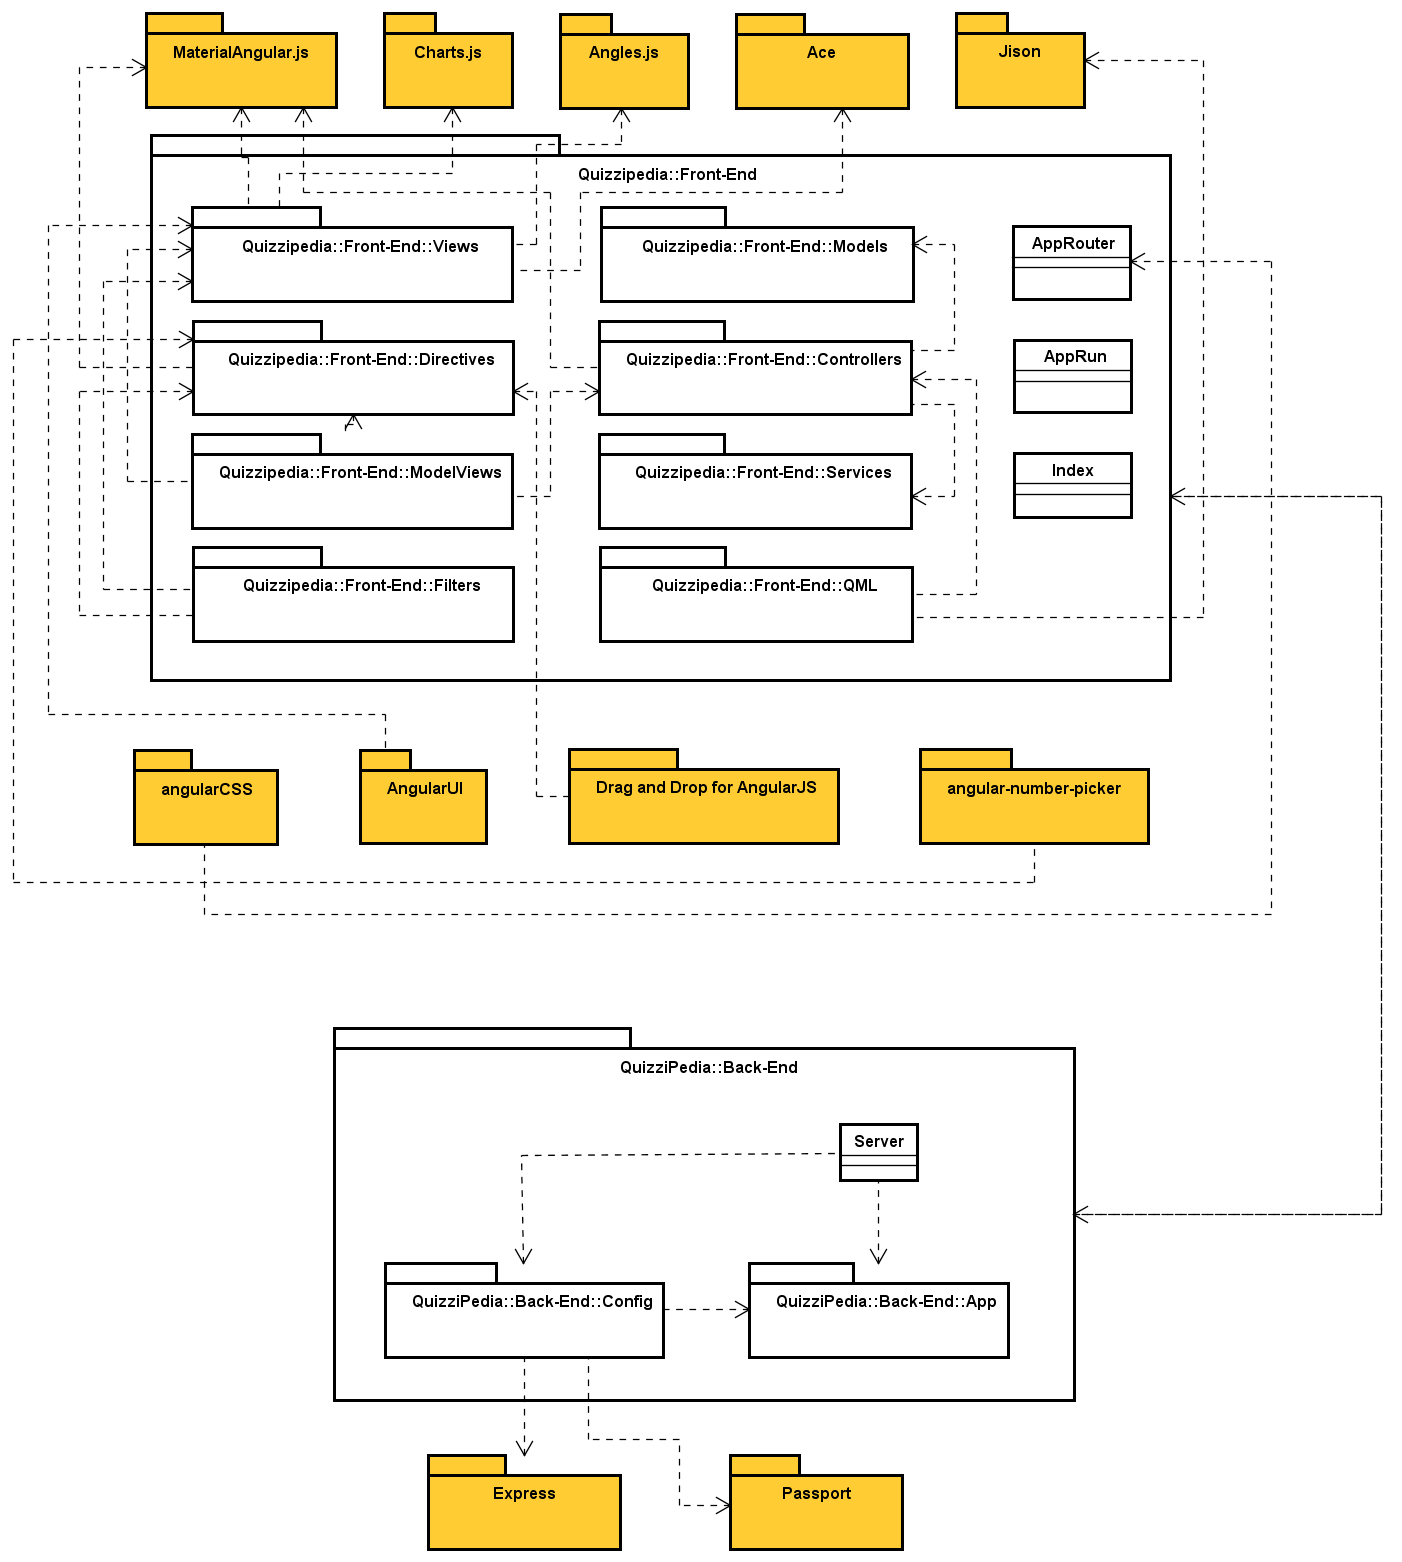
\includegraphics[scale=0.35]{UML/Package/QuizziPedia.png}
	\caption{Architettura}
\end{figure}
\FloatBarrier
\begin{itemize}
	\item \textbf{Descrizione}: architettura ad alto livello dell'applicazione \progetto;
	\item \textbf{Packages contenuti}:
	\begin{itemize}
		\item \texttt{QuizziPedia::Front-End}: \textit{package\ped{G}} contenente i \textit{packages\ped{G}} che compongono il Front-End;
		\item \texttt{QuizziPedia::Back-End}: \textit{package\ped{G}} contenente i \textit{packages\ped{G}} che compongono il Back-End;
		\item \texttt{MaterialAngular.js}: framework per lo sviluppo dei componenti grafici dell'applicazione;
		\item \texttt{Charts.js}: libreria per lo sviluppo dei grafici per la visualizzazione delle statistiche utente;
		\item \texttt{Angles.js}: libreria necessaria per integrare la libreria Charts.js all'interno dell'ambiente \textit{Angular\ped{G}};
		\item \texttt{TextAngular.js}: libreria per la creazione di un editor di testo all'interno delle pagine web per permettere all'utente di creare domande custom in linguaggio \textit{QML\ped{G}};
		\item \texttt{Jison}: è un generatore di parser JavaScript;
		\item \texttt{Express}: framework Web di routing e middleware, con funzionalità sua propria minima: un’applicazione Express è essenzialmente una serie di chiamate a funzioni middleware;
		\item \texttt{Passport}: \textit{middleware\ped{G}} per l'autenticazione in ambiente \textit{Node.js\ped{G}}.
	\end{itemize}
\end{itemize}

\newpage
\section{QuizziPedia::Front-End}
\label{QuizziPedia::Front-End}
\begin{figure}[ht]
	\centering
	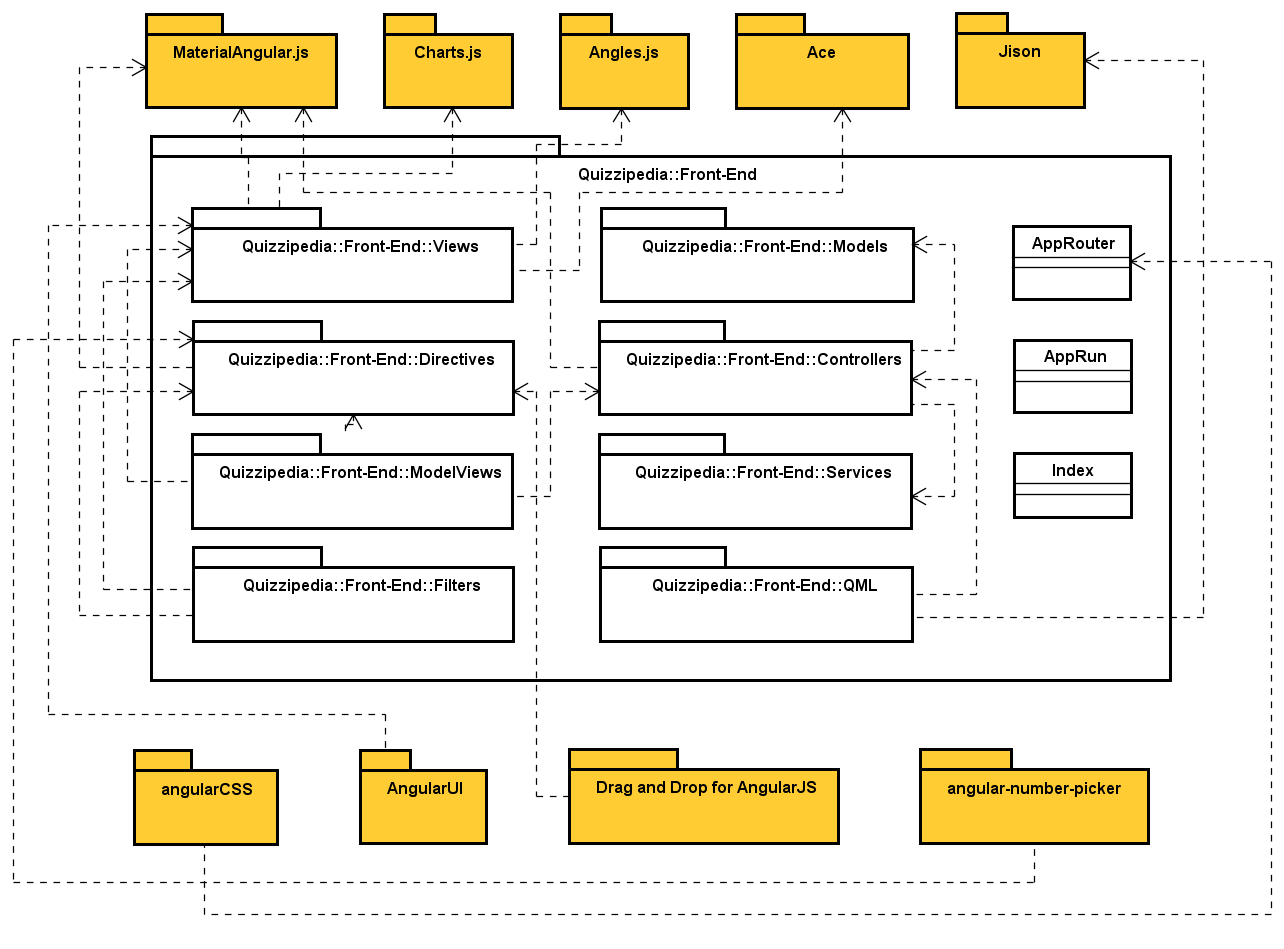
\includegraphics[scale=0.35]{UML/Package/QuizziPedia_Front-end.png}
	\caption{QuizziPedia::Front-End}
\end{figure}
\FloatBarrier
\begin{itemize}
	\item \textbf{Descrizione}: \textit{package\ped{G}} contenente le componenti front-end dell'applicazione;
	\item \textbf{Package contenuti}:
	\begin{itemize}
		\item \texttt{Views}: \textit{package\ped{G}} contenente le \textit{views\ped{G}} front-end dell'applicazione;
		\item \texttt{Controllers}: \textit{package\ped{G}} contenente i \textit{controllers\ped{G}} front-end dell'applicazione;
		\item \texttt{Services}: \textit{package\ped{G}} contenente i \textit{services\ped{G}} front-end dell'applicazione;
		\item \texttt{Models}: \textit{package\ped{G}} contenente le classi che definiscono la business logic dell'applicazione;
		\item \texttt{Directives}: \textit{package\ped{G}} contenente le \textit{directives\ped{G}} front-end dell'applicazione.
	\end{itemize}
	\item \textbf{Classi contenute}:
	\begin{itemize}
		\item \texttt{Index}: \textit{view\ped{G}} generale dell'applicazione. Contiene gli elementi che saranno presenti in ogni pagina dell'applicazione;
		\item \texttt{AppRun}: classe che verifica se l'utente sia autenticato e che abbia le giuste autorizzazioni per la pagina in cui si trova;
		\item \texttt{AppRouter}: classe che gestisce i routes dell'applicazione, utilizza il servizio \$routeProvider per associare ad ogni route un \textit{controller\ped{G}} e una \textit{view\ped{G}}.
	\end{itemize}
\end{itemize}

\newpage
\subsection{QuizziPedia::Front-End::Views}

\label{QuizziPedia::Front-End::Views}
\begin{figure}[ht]
	\centering
	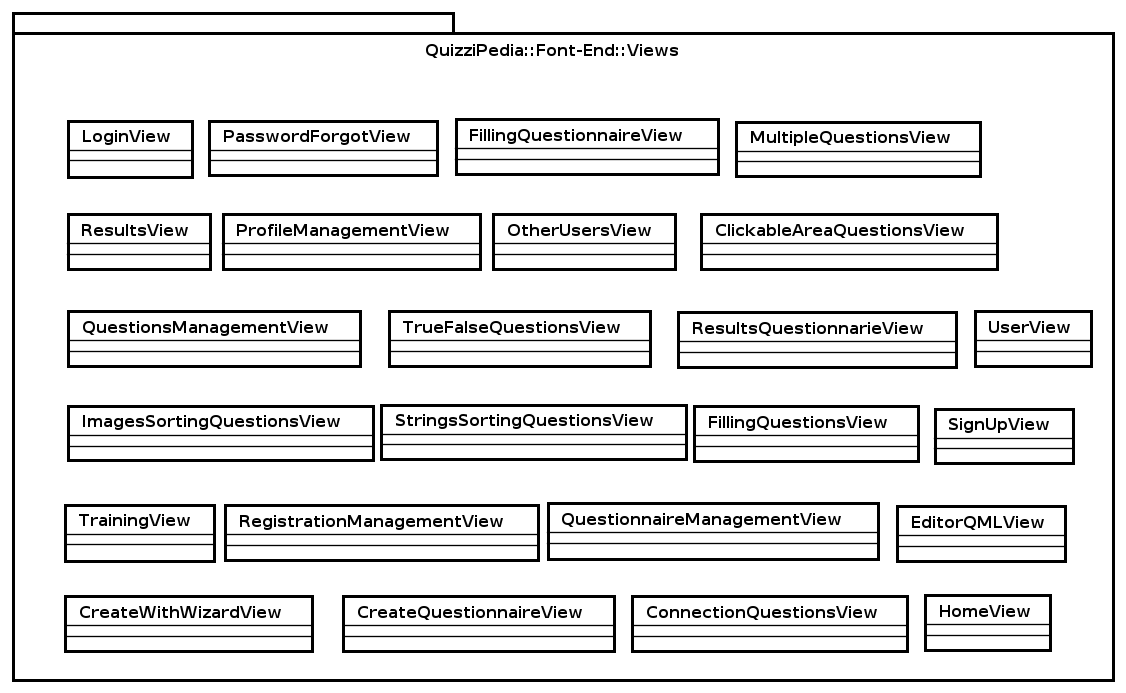
\includegraphics[scale=0.55]{UML/Package/QuizziPedia_Front-End_Views.png}
	\caption{QuizziPedia::Front-End::Views}
\end{figure}\FloatBarrier
\begin{itemize}
	\item \textbf{Descrizione}: package contenente le views front-end dell'applicazione;
	\item \textbf{Padre}: \texttt{Front-End};
	\item \textbf{Interazione con altri componenti}:
	\begin{itemize}
		\item \texttt{Controllers}: package contenente i \textit{controllers\ped{G}} Front-End dell'applicazione;
		\item \texttt{Directives}: package contenente le \textit{directives\ped{G}} Front-End dell'applicazione.
	\end{itemize}
	\item \textbf{Classi contenute}:
	\begin{itemize}
		\item \texttt{LoginView}: classe contenente le form necessarie per effettuare il login. Contiene inoltre un link alla pagina di registrazione e uno alla pagina per il recupero della password;
		\item \texttt{SignUpView}: classe contenente le form dedicate alla registrazione utente. Contiene inoltre un link alla pagina di login;
		\item \texttt{PasswordForgotView}: classe contenente le form necessarie per il recupero della password dimenticata;
		\item \texttt{HomeView}: classe contenente la direttiva per barra di ricerca degli utenti e questionari e il bottone che porterà l'utente nella modalità allenamento;
		\item \texttt{ResultsView}: classe contenente i risultati della ricerca effettuata. Vengono visualizzati sia gli utenti che i questionari trovati;
		\item \texttt{UserView}: contenente le direttive dei dati personali dell'utente, delle sue statistiche relative ai questionari e agli allenamenti effettuati e dei questionari a cui è iscritto;
		\item \texttt{OtherUserView}: classe contenente le direttive dei dati personali e delle statistiche di un utente ricercato;
		\item \texttt{ProfileManagementView}: classe contenente i dati personali che un utente può modificare dopo essersi registrato al sistema;
		\item \texttt{QuestionsManagementView}: classe contenente l'elenco delle domande create;
		\item \texttt{TrueFalseQuestionView}: classe contenente le direttive per creare una domanda vero/falso;
		\item \texttt{MultipleQuestionView}: classe contenente le direttive per creare una domanda a risposta multipla;
		\item \texttt{ConnectionQuestionView}: classe contenente i campi e le direttive per creare una domanda a collegamento;
		\item \texttt{ImagesSortingQuestionView}: classe contenente i campi e le direttive per creare una domanda a ordinamento immagini;
		\item \texttt{StringsSortingQuestionView}: classe contenente i campi e le direttive per creare una domanda a ordinamento stringhe;
		\item \texttt{FillingQuestionsView}: classe contenente i campi e le direttive per creare una domanda a riempimento testo;
		\item \texttt{ClickableAreaQustionView}: classe contenente i campi e le direttive per creare una domanda ad area cliccabile;
		\item \texttt{EditorQMLView}: classe contenente l'editor \textit{QML\ped{G}} per la creazione di domande personalizzate;
		\item \texttt{TrainingView}: classe principale della modalità allenamento; conterrà i vari templates di ogni domanda dell'allenamento;
		\item \texttt{FillingQuestionnaireView}: classe principale per la compilazione del questionario; conterrà i vari templates di ogni domanda appartenente al questionario;
		\item \texttt{QuestionnaireManagementView}: classe principale per la gestione dei questionari;
		\item \texttt{CreateQuestionnaireView}: classe per la creazione del questionario;
		\item \texttt{ResultQuestionnaireView}: classe contenente i risultati conseguiti dagli utenti che hanno compilato il proprio questionario;
		\item \texttt{RegiastrationManagementView}: classe che permette di visualizzare gli utenti iscritti ad un questionario.
	\end{itemize}
\end{itemize}
\newpage
\subsection{QuizziPedia::Front-End::Controllers}

\begin{figure} [ht]
	\centering
	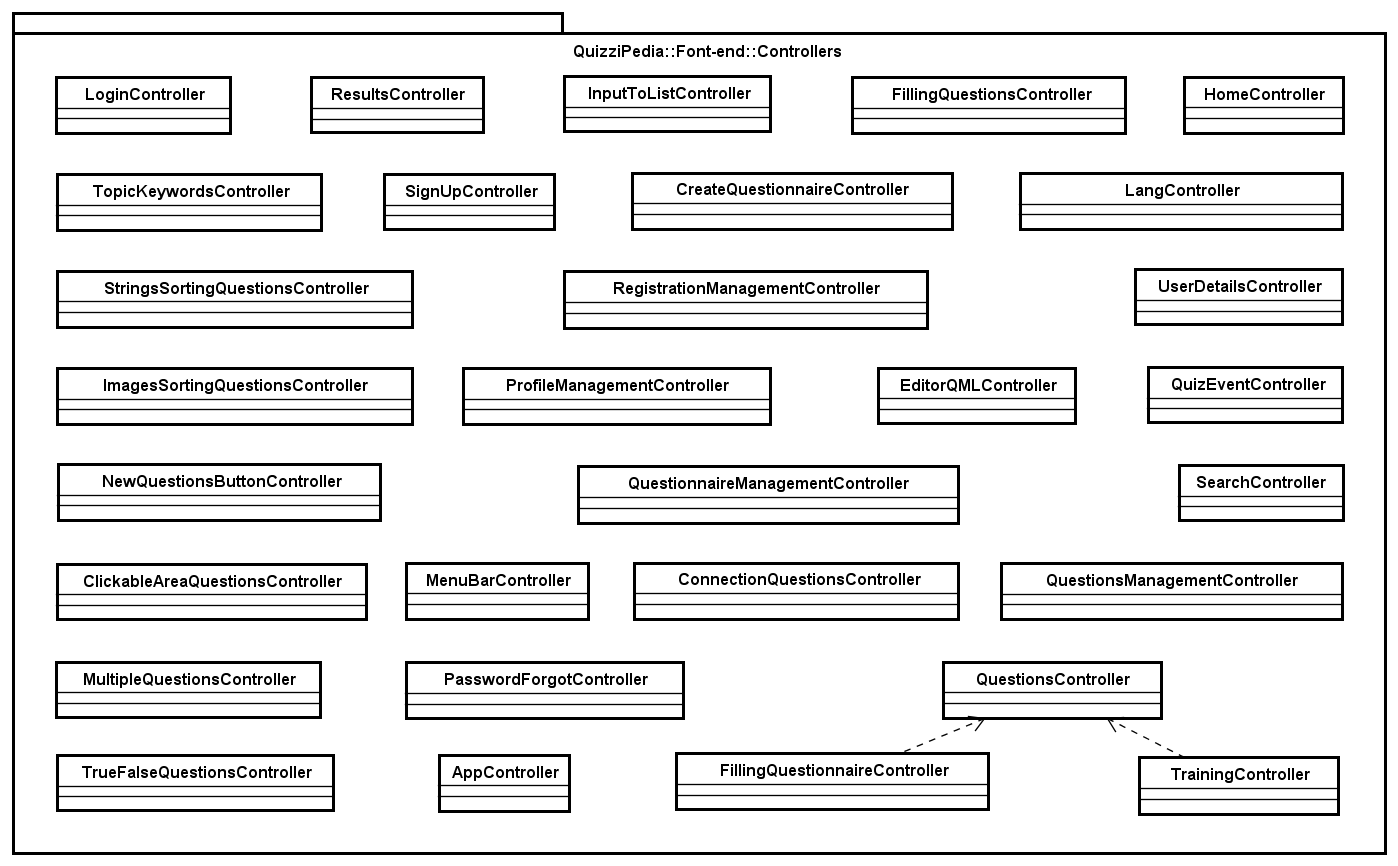
\includegraphics[scale=0.45]{UML/Package/QuizziPedia_Front-End_Controllers.png}
	\caption{QuizziPedia::Front-End::Controllers}
\end{figure} \FloatBarrier

\begin{itemize}
	\item \textbf{Descrizione}: \textit{package\ped{G}} che contiene i controller individuati per la parte front-end dell'applicazione;
	\item \textbf{Padre}: \texttt{Front-End};
	\item \textbf{Interazione con altri componenti}:
	\begin{itemize}
		\item \texttt{Views}: \textit{package\ped{G}} che contiene le \textit{views\ped{G}} dell'applicazione;
		\item \texttt{Models}: \textit{package\ped{G}} che contiene le classi \textit{model\ped{G}} dell'applicazione;
		\item \texttt{Services}: \textit{package\ped{G}} che contiene i \textit{services\ped{G}} dell'applicazione.
	\end{itemize}
	\item \textbf{Classi contenute}:
	\begin{itemize}
		\item \texttt{ClickableAreaQuestionController}: questa classe permette di gestire la creazione e la modifica di una domanda ad area cliccabile;
		\item \texttt{ConnectionQuestionController}: questa classe permette di gestire la creazione e la modifica di una domanda a collegamento;
		\item \texttt{CreateQuesrtionnaireController}: questa classe permette di gestire la creazione di un questionario;
		\item \texttt{EditorQMLController}: questa classe permette di gestire la creazione e la modifica di domande create tramite editor \textit{QML\ped{G}};
		\item \texttt{FillingQuestionnaireController}: questa classe permette di gestire la compilazione del questionario;
		\item \texttt{FillingQuestionsController}: questa classe permette di gestire la creazione e la modifica di una domanda	a riempimento di spazi;
		\item \texttt{HomeController}: questa classe permette di gestire la home page;
		\item \texttt{ImagesSortingQuestionsController}: questa classe permette di gestire la creazione e la modifica di una domanda a ordinamento immagini;
		\item \texttt{InputToListController}: questa classe permette di gestire l'inserimento di una lista di risposte durante la creazione di una domanda;
		\item \texttt{LoginController}: questa classe permette di gestire l'autenticazione dell'utente al sistema;
		\item \texttt{MenuBarController}: questa classe permette di gestire il menù fisso per ogni pagina;
		\item \texttt{MultipleQuestionController}: questa classe permette di gestire la creazione e la modifica di una domanda a risposta multipla;
		\item \texttt{NewQuestionButtonController}: questa classe permette di effettuare il redirect alla pagina di creazione nuova domanda;
		\item \texttt{PasswordForgotController}: questa classe permette di gestire il ripristino della password dimenticata;
		\item \texttt{ProfileManagementController}: questa classe permette di gestire il profilo personale di un utente;
		\item \texttt{QuestionnaireDeatailsController}: questa classe permette di gestire i dettagli di un questionario;
		\item \texttt{QuestionnaireManagementController}: questa classe permette di gestire tutti i questionari creati da un utente;
		\item \texttt{QuestionsController}: questa classe permette di gestire il recupero delle domande per far si che possano essere visualizzate nella modalità allenamento e nella compilazione dei questionari;
		\item \texttt{QuestionsManagementController}: questa classe permette di gestire le domande create dall'utente e di crearne di nuove;
		\item \texttt{QuizEventController}: questa classe permette di reagire ai comandi dell'utente durante la gestione dei suoi questionari;
		\item \texttt{RegistrationManagementController}: questa classe permette di gestire le iscrizione degli utenti ai questionari;
		\item \texttt{ResultQuestionnaireController}: questa classe permette di gestire la visualizzazione dei risultati di un singolo questionario;
		\item \texttt{SearchController}: questa classe permette di gestire la ricerca di questionari e utenti all'interno dell'applicazione;
		\item \texttt{SignUpController}: questa classe permette di gestire la registrazione di un utente al sistema;
		\item \texttt{StatisticsController}: questa classe permette di gestire le statistiche di un utente;
		\item \texttt{StringsSortingQuestionController}: questa classe permette di gestire la creazione e la modifica di una domanda a ordinamento di stringhe;
		\item \texttt{TopicKeywordsController}: questa classe permette di gestire il recupero delle parole chiave di un questionario;
		\item \texttt{TrainingController}: questa classe permette di gestire la modalità allenamento sottoponendo all'utente le giuste domande adatte al suo livello;
		\item \texttt{TrueFalseQuestionController}: questa classe permette di gestire la creazione e la modifica di una domanda	vero/falso;
		\item \texttt{UserDetailsController}: questa classe permette di gestire i dati di un utente da mostrare nella pagina di un profilo.
	\end{itemize} 
\end{itemize}
\newpage
\subsection{QuizziPedia::Front-End::Services}
\begin{figure}[ht]
	\centering
	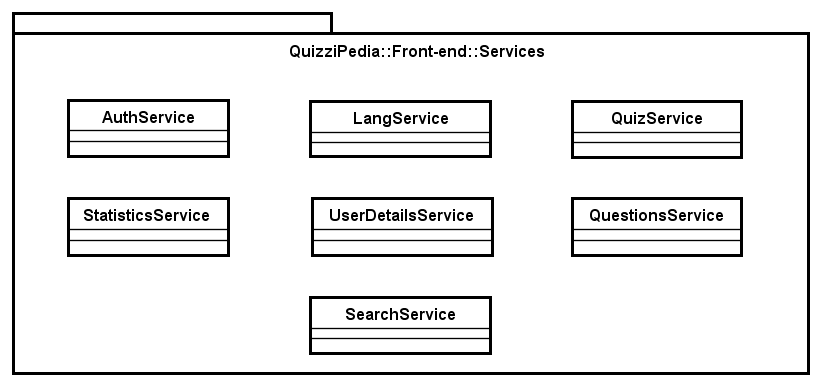
\includegraphics[scale=0.55]{UML/Package/QuizziPedia_Front-End_Services.png}
	\caption{QuizziPedia::Front-End::Services}
\end{figure} \FloatBarrier

\begin{itemize}
	\item \textbf{Descrizione}: package che contiene le classi individuate che permettono la comunicazione del lato front-end con il lato back-end;
	\item \textbf{Padre:} \texttt{Front-End};
	\item \textbf{Interazione con altri componenti:}
	\begin{itemize}
		\item \texttt{Models}: package che contiene le classi \textit{model\ped{G}} dell'applicazione;
		\item \texttt{Controllers}: package che contiene le classi \textit{controller\ped{G}} dell'applicazione.
	\end{itemize}
	\item \textbf{Classi contenute}:
	\begin{itemize}
		\item \texttt{AuthServices}: questa classe permette di gestire la registrazione e l'autenticazione di un utente;
		\item \texttt{LangService}: questa classe permette di gestire la lingua nella quale si è scelto di utilizzare l'applicazione;
		\item \texttt{QuestionsService}: questa classe permette di ottenere domande esistenti e salvare nuove domande;
		\item \texttt{QuizService}: questa classe permette di ottenere i dati di un quiz tramite delle parole chiave inserite dall'utente nella barra di ricerca. Permette inoltre di iscriversi ad un questionario e di scaricare l'intera lista di domande di un questionario a partire dal suo id univoco;
		\item \texttt{SearchService}: questa classe permette di gestire il recupero dei dati dal back-end a seguito di una ricerca effettuata da un utente;
		\item \texttt{StatisticsService}: questa classe permette di ottenere le statistiche dell'utente;
		\item \texttt{UserDetailsService}: questa classe permette di ottenere i dati personali degli utenti.
	\end{itemize} 
\end{itemize}
\newpage

\subsection{QuizziPedia::Front-End::Directives}

\label{QuizziPedia::Front-End::Directives}
\begin{figure} [ht]
	\centering
	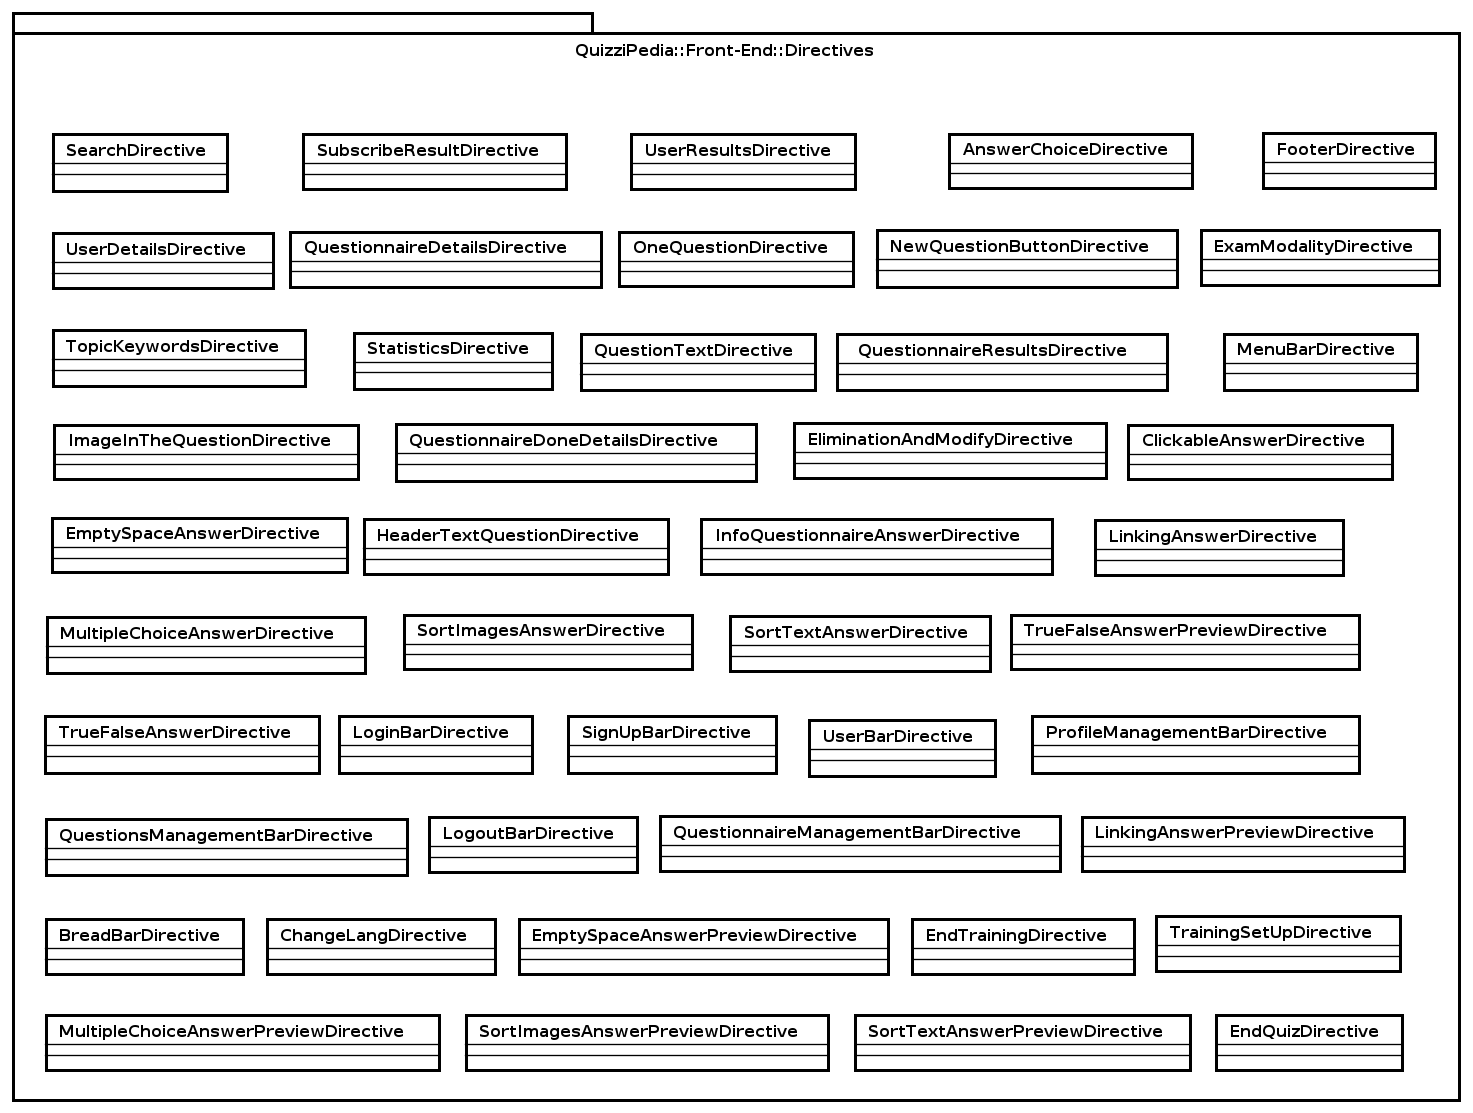
\includegraphics[scale=0.40]{UML/Package/QuizziPedia_Front-End_Directives.png}
	\caption{QuizziPedia::Front-End::Directives}
\end{figure}

\begin{itemize}
	\item \textbf{Descrizione}: package contenente le \textit{directives\ped{G}};
	\item \textbf{Padre}: \texttt{Front-End};
	\item \textbf{Interazione con altri componenti}:
	\begin{itemize}
		\item \texttt{Controllers}: package contenente i \textit{controllers\ped{G}} front-end dell'applicazione;
		\item \texttt{Views}: package contenente le \textit{views\ped{G}} front-end dell'applicazione.
	\end{itemize}
	\item \textbf{Classe contenute}:
	\begin{itemize}
		\item \texttt{EliminationAndModifyDirective}: componente grafico contenente i bottoni per eliminare o modificare un questionario;
		\item \texttt{ExamModalityDirective}: classe contenete i componenti grafici per attivare la modalità esame su un questionario e gestire le iscrizioni;
		\item \texttt{FooterDirective}: classe contenente i componenti grafici del footer dell'applicazione;
		\item \texttt{ImageInTheQuestionDirective}: classe contenente i componenti grafici per l'inserimento dell'immagine	nella creazione delle domande;
		\item \texttt{MenuBarDirective}: rappresenta il menù, presente in ogni pagina dell'applicazione, generato in base agli oggetti passati nello \$scope isolato. Fornisce un pulsante per ogni oggetto ricevuto come parametro, ogni pulsante viene rappresentato con un'icona e con un testo. Al click di un pulsante viene invocata la funzione ad esso associata;
		\item \texttt{OneQuestionDirective}: rappresenta il componente grafico che visualizza all'utente l'anteprima della domanda che ha creato. Eseguendo l'azione di click sul pulsante di modifica sarà possibile modificare tale domanda. All'interno di QuestionsManagementsView verranno stampati a video tanti componenti quanti presenti nello \$scope isolato ad esso associato;
		\item \texttt{NewQuestionButtonDirective}: rappresenta il componente grafico che permette all'utente di posizionarsi nella \textit{view\ped{G}} di creazione di una nuova domanda;
		\item \texttt{QuestionTextDirective}: rappresenta il componente grafico che permette all'utente di scrivere o modificare il testo di una domanda;
		\item \texttt{QuestionnaireDetailsDirective}: rappresenta il componente grafico che permette all'utente di visualizzare la lista di questionari che può compilare;
		\item \texttt{QuestionnaireDoneDetailsDirective}: rappresenta il componente grafico che permette all'utente di visualizzare la lista di questionari che ha già compilato e di conseguenza vederne le valutazioni;
		\item \texttt{QuestionnaireResultsDirective}: rappresenta il componente grafico che permette all'utente autenticato pro di vedere i risultati di chi ha compilato il questionario. Tale componente è contenuto nella lista dei questionari abilitati alla compilazione. É possibile accedere alla lista dei risultati azionando l'evento ad esso collegato;
		\item \texttt{QuestionnaireResultsDirective}: rappresenta il componente grafico che permette all'utente autenticato pro di vedere i risultati di chi ha compilato il questionario. Tale componente è contenuto nella lista dei questionari abilitati alla compilazione. É possibile accedere alla lista dei risultati azionando l'evento ad esso collegato;
		\item \texttt{SearchDirective}: classe che permette di effettuare la ricerca di utenti e questionari;
		\item \texttt{StatisticsDirective}: classe che permette di visualizzare le statistiche di un utente;
		\item \texttt{SubscribeResultDirective}: classe che permette di visualizzare e iscriversi ai questionari ricercati;
		\item \texttt{TopicKeywordsDirective}: classe che permette di gestire l'inserimento dell'argomento e delle	keywords al momento della creazione della domanda;
		\item \texttt{UserDetailsDirective}: classe che permette di visualizzare i dati personali di un utente;
		\item \texttt{UserResultsDirective}: classe che permette di visualizzare la lista degli utenti ricercati dopo aver utilizzato l'apposita funzione di ricerca;
		\item \texttt{ClickableAnswerDirective}: rappresenta il componente grafico che permette all'utente di visualizzare la domanda ad area cliccabile nell'immagine;
		\item \texttt{EmptySpaceAnswerDirective}: rappresenta il componente grafico che permette all'utente di visualizzare l'esercizio a riempimento di spazi vuoti;
		\item \texttt{HeaderTextQuestionDirective}: rappresenta componente grafico che presenta all'utente l'argomento e le parole chiave della domanda che ha a schermo;
		\item \texttt{InfoQuestionnaireDirective}: rappresenta il componente grafico che permette all'utente di visualizzare le informazioni principali del questionario che si sta per svolgere;
		\item \texttt{LinkingAnswerDirective}: rappresenta componente grafico che permette all'utente di visualizzare la domanda di collegamento;
		\item \texttt{MultipleChoiceAnswerDirective}: rappresenta componente grafico che permette all'utente di visualizzare la domanda a risposta multipla;
		\item \texttt{SortImagesAnswerDirective}: rappresenta il componente grafico che permette all'utente di visualizzare la domanda ad ordinamento di immagini;
		\item \texttt{SortTextAnswerDirective}: rappresenta il componente grafico che permette all'utente di visualizzare la domanda ad ordinamento di stringhe;
		\item \texttt{TrainingSetUpDirective}: rappresenta componente grafico che permette all'utente di selezionare l'argomento e le parole chiave per iniziare un allenamento con queste caratteristiche;
		\item \texttt{TrueFalseAnswerDirective}: rappresenta il componente grafico che permette all'utente di visualizzare la domanda vero e falso;
		\item \texttt{LoginBarDirective}: directive contenente il componente che permette di effettuare il redirect alla pagina di login;
		\item \texttt{SignUpBarDirective}: directive contenente il componente che permette di effettuare il redirect alla pagina di registrazione;
		\item \texttt{UserBarDirective}: directive contenente il componente che permette di effettuare il redirect alla pagina di visualizzazione profilo;
		\item \texttt{ProfileManagementBarDirective}: directive contenente il componente che permette di effettuare il redirect alla pagina di gestione del profilo;
		\item \texttt{QuestionsManagementBarDirective}: directive contenente il componente che permette di effettuare il redirect alla pagina di gestione delle domande;
		\item \texttt{LogoutBarDirective}: directive contenente il componente che permette di effettuare il logout dal sistema;
		\item \texttt{QuestionnaireManagementBarDirective}: directive contenente il componente che permette di effettuare il redirect alla pagina di gestione dei questionari.
	\end{itemize}
\end{itemize}
%\newpage

\subsection{QuizziPedia::Front-End::Models}

	\label{QuizziPedia::Front-End::Models}
	
	\begin{figure}[ht]
		\centering
		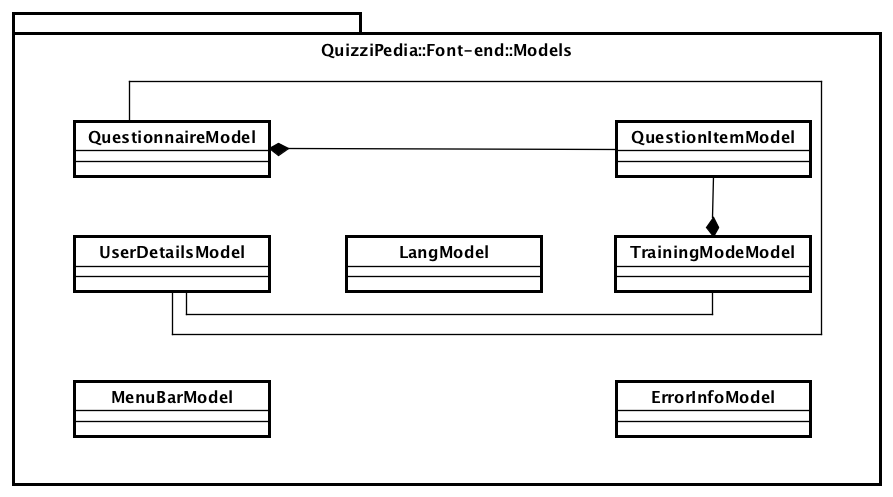
\includegraphics[scale=0.5,keepaspectratio]{UML/Package/QuizziPedia_Front-End_Models.png}
		\caption{QuizziPedia::Front-End::Models}
	\end{figure} \FloatBarrier

		\begin{itemize}
			\item \textbf{Descrizione}: \textit{package\ped{G}} contenente le classi che definiscono la business logic dell'applicazione;
			\item \textbf{Padre}: \texttt{Front-End};
			\item \textbf{Iterazioni con altri componenti}: 
				\begin{itemize}				
					\item \texttt{Controllers}: \textit{package\ped{G}} contenente i controllers front-end dell'applicazione;
					\item \texttt{Directives}: \textit{package\ped{G}} contenente le directives front-end dell'applicazione;
					\item \texttt{Models}: \textit{package\ped{G}} contenente le classi che definiscono la business logic dell'applicazione;
					\item \texttt{Services}: \textit{package\ped{G}} che contiene le classi individuate che permettono la comunicazione del lato front-end con il lato back-end attraverso l'architettura \textit{REST\ped{G}}.
				\end{itemize}
			\item \textbf{Classi contenute}:
			\begin{itemize}
				\item \texttt{UserDetailsModel}: rappresenta un utente. Contiene tutte le informazioni necessarie alla presentazione del contenuto di un utente sia nella visualizzazione che nella gestione di un profilo;
				\item \texttt{TrainingModeModel}: rappresenta un allenamento. Contiene tutte le informazioni necessarie alla presentazione del contenuto di un allenamento;
				\item \texttt{QuestionnaireModel}: rappresenta un questionario. Contiene tutte le informazioni necessarie alla presentazione del contenuto del questionario;
				\item \texttt{QuestionItemModel}: rappresenta una domanda. Contiene tutte le informazioni necessarie alla presentazione del contenuto della domanda;
				\item \texttt{MenuBarModel}: questa classe racchiude i dati necessari per la creazione dinamica della barra menù posizionata in modo fisso su ogni pagina;
				\item \texttt{LangModel}: rappresenta le informazioni per la giusta traduzione dell'applicazione;
				\item \texttt{ErrorInfoModel}: rappresenta le informazioni di un errore che si è verificato eseguendo una determinata operazione;
			\end{itemize}
		\end{itemize}

\newpage
\section{Specifica del Back-End}
\subsection{QuizziPedia::Back-End}
\subsubsection{Informazioni generali}
\label{QuizziPedia::Back-End}
\begin{figure}
	\centering
	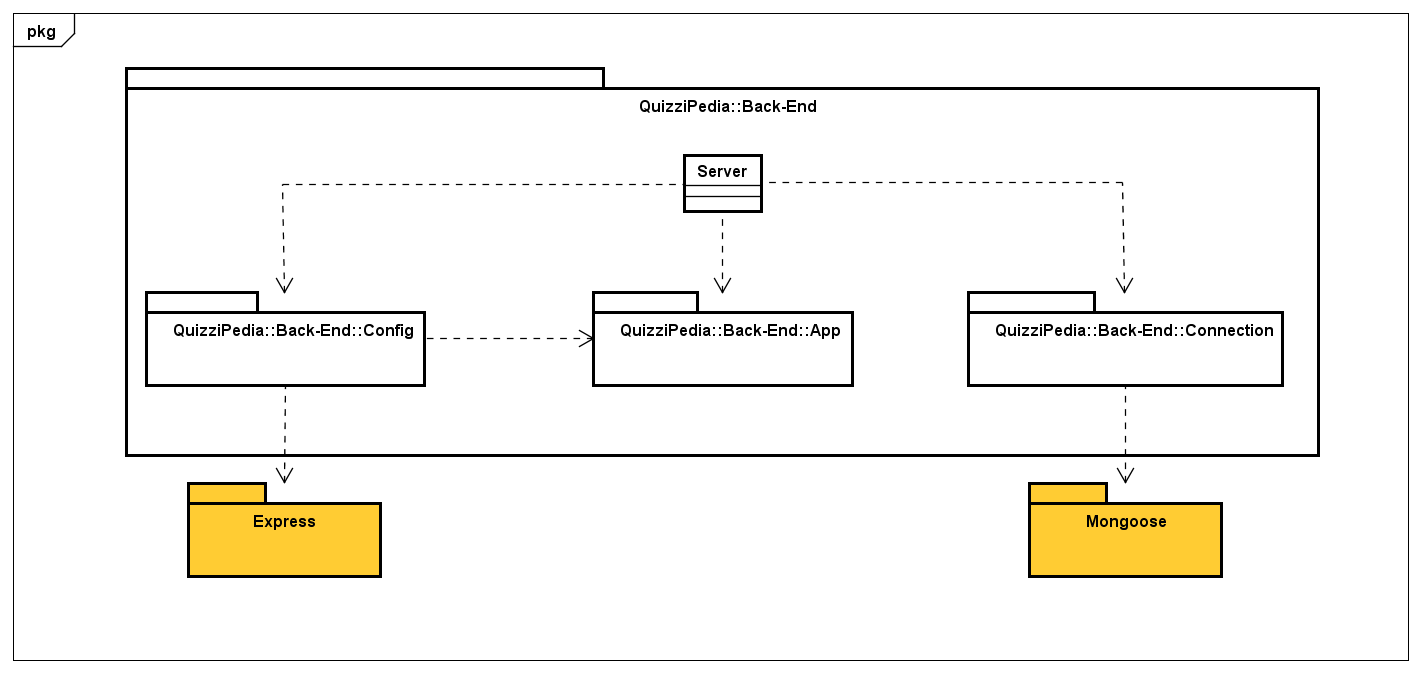
\includegraphics[scale=0.45]{UML/Package/QuizziPedia_Back-End.png}
	\caption{QuizziPedia::Back-End}
\end{figure}

	\begin{itemize}
		\item \textbf{Descrizione} \\ Package contenenti le componenti della parte back-end dell' applicazione.
		\item \textbf{Package contenuti}
		\begin{itemize}
			\item App \\
			Package\ped{G} contenente le componenti del server che implementano il \textit{pattern MVC\ped{G}}.
			\item Config \\
			Package\ped{G} contenente le componenti di configurazione del server\ped{G}.
		\end{itemize}
	\end{itemize}
\subsubsection{Classi}
	\paragraph{QuizziPedia::Back-End::Server}
	\begin{itemize}
		\item \textbf{Descrizione}
		\item \textbf{Utilizzo}
		\item \textbf{Relazioni con altre classi}
		\item \textbf{Attributi}
		\item \textbf{Metodi}
	\end{itemize}

\subsection{QuizziPedia::Back-End::Connection}
\subsubsection{Informazioni generali}
\subsubsection{Classi}

\subsection{QuizziPedia::Back-End::App}
\subsubsection{Informazioni generali}
\label{QuizziPedia::Back-End::App}
\begin{figure}
	\centering
	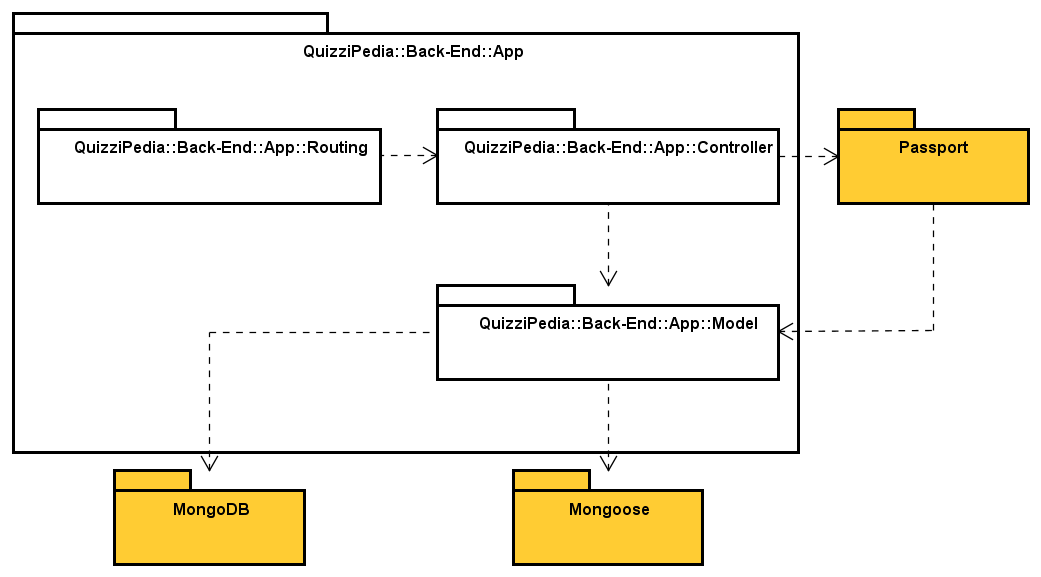
\includegraphics[scale=0.45]{UML/Package/QuizziPedia_Back-End_App.png}
	\caption{QuizziPedia::Back-End::App}
\end{figure}
	\begin{itemize}
		\item \textbf{Descrizione} \\
		Package contenente le componenti del server che implementano il \textit{pattern\ped{G} MVC\ped{G}};
		\item \textbf{Padre} \\ Back-End;
		\item \textbf{Interazioni con altri componenti}
			\begin{itemize}
				\item Congif \\
				Package contenente le componenti di configurazione del server;
			\end{itemize}
		\item \textbf{Package contenuti}
			\begin{itemize}
				\item Controllers \\
				Package che contiene i controllers di Express, definisce la logica dell'applicazione;
				\item Models \\
				Package che contiene le classi che definiscono il model dell'applicazione. Queste classi cono definite come classi schema di \textit{Mongoose\ped{G}}, il quale permette di utilizzare \textit{MongoDB\ped{G}} tramite degli oggetti;
				\item Routers \\
				Package contenente i routers della componente back-end dell'applicazione. Contiene i file di configurazione relativi al routing delle richieste del client, ossia i routers di Express.
			\end{itemize}
	\end{itemize}
	
\subsection{QuizziPedia::Back-End::App::Controllers}
\subsubsection{Informazioni generali}
	\begin{itemize}
		\item \textbf{Descrizione} \\
		\item \textbf{Padre} \\
		\item \textbf{Interazioni con altri componenti} \\
		\item \textbf{Package contenuti}
	\end{itemize}
\subsubsection{Classi}
\paragraph{QuizziPedia::Back-End::App::Controllers::NOMECLASSE}
	\begin{itemize}
		\item \textbf{Descrizione} \\
		\item \textbf{Utilizzo} \\
		\item \textbf{Relazioni con altre classi} \\
		\item \textbf{Metodi} \\
	\end{itemize}


\subsection{QuizziPedia::Back-End::App::Models}
\subsubsection{Informazioni generali}
\subsubsection{Classi}
\paragraph{QuizziPedia::Back-End::App::Models::NOMECLASSE}
\begin{itemize}
	\item \textbf{Descrizione} \\
	\item \textbf{Utilizzo} \\
	\item \textbf{Relazioni con altre classi} \\
	\item \textbf{Metodi} \\
\end{itemize}

\subsection{QuizziPedia::Back-End::App::Routers}
\subsubsection{Informazioni generali}
\subsubsection{classi}
\paragraph{QuizziPedia::Back-End::App::Routers::NOMECLASSE}
	\begin{itemize}
		\item \textbf{Descrizione} \\
		\item \textbf{Utilizzo} \\
		\item \textbf{Relazioni con altre classi} \\
		\item \textbf{Metodi} \\
<<<<<<< HEAD
	\end{itemize}
=======
	\end{itemize}
>>>>>>> origin/master

\newpage
\section{Estensione delle funzionalità}
Per ragioni di tempo e di competenze, alcune funzionalità del software \progetto{} non sono state implementate. In questo capitolo vengono elencati tutti i punti di possibile estensione delle funzionalità e un loro possibile sviluppo.
\subsection{Autenticazione tramite social network}
Uno degli obbiettivi principali dell'applicazione \progetto{} è quello della condivisione di domande e questionari. E' stata perciò progettata e sviluppata per essere un software social e conforme alle ultime tendenze grafiche. Per questo, uno dei requisiti desiderabili è permettere all'utente di non perdere tempo durante la fase di registrazione, ma di poterlo fare appoggiandosi alle ultime piattaforme social come Facebook e Twitter. Il \textit{framework\ped{G}} Passport utilizzato del team per le funzionalità di registrazione e autenticazione, permette nativamente di implementare la registrazione tramite i più famosi social network attuali. La guida per implementare queste funzionalità si trova alla pagina \url{http://passportjs.org/docs}. 
\subsection{Cambio tipologia account}
Le tipologie di utenza dell'applicazione \progetto{} sono principalmente tre:
\begin{itemize}
	\item Utente non autenticato;
	\item Utente autenticato;
	\item Utente autenticato pro.
\end{itemize}
La tipologia di utente autenticato pro è stata pensata principalmente per i professori universitari e delle scuole medie/superiori che vogliono appoggiarsi alla piattaforma \progetto{} per creare questionari finalizzati alle verifiche e agli esami. Allo stato attuale, l'applicazione permette il passaggio da utente normale a pro semplicemente cliccando l'apposito pulsante presente all'interno della pagina \textit{Gestione profilo}. In base alle esigenze strategiche ed economiche dell'azienda acquirente di \progetto{}, sarà opportuno sviluppare ulteriormente questa funzionalità di cambio tipologia account, ad esempio associando un metodo di pagamento oppure l'immissione di un particolare codice che solo i professori associati a scuole e università possono avere.  
\subsection{Creazione delle domande tramite wizard}
La creazione delle domande avviene tramite il linguaggio di markup QML (si veda l'Appendice A). Esso è stato creato per essere semplice e comprensibile ma allo stesso tempo molto potente. Permette infatti di creare non solo domande classiche come vero/falso, a scelta multipla e ordinamento, ma anche di combinare questi generi tra loro e creare così nuove tipologie di domande. Questo ha causato un piccolo aumento della difficoltà del linguaggio che potrebbe risultare poco attraente ad un utente con poca famigliarità con i linguaggi di programmazione. Per ovviare questo problema è opportuno sviluppare una nuova modalità di creazione delle domande tramite wizard guidati. Le tipologie base delle domande sviluppate allo stato attuale sono sei:
\begin{itemize}
	\item Vero/Falso;
	\item Risposta multipla;
	\item Ordinamento stringhe;
	\item Ordinamento immagini;
	\item Riempimento spazi vuoti;
	\item Collegamento stringhe.
\end{itemize}
Lo sviluppo di wizard per la creazione di ogni tipologia di domanda base, aiuterebbe l'utente medio, che non ha famigliarità con i linguaggi di markup, nell'utilizzo del servizio \progetto.   
\subsection{Nuove tipologie di domande}
Il linguaggio QML (si veda l'Appendice A) prevede sei tipologie di domande base:
\begin{itemize}
	\item Vero/Falso;
	\item Risposta multipla;
	\item Ordinamento stringhe;
	\item Ordinamento immagini;
	\item Riempimento spazi vuoti;
	\item Collegamento stringhe.
\end{itemize}
E' possibile estendere il codice per creare nuove tipologie di domande base. Questo prevede l'aggiunta di una nuova classe con il relativo codice QML all'interno del package \texttt{questionCheck} e aggiornare la classe \texttt{CheckQML} con la nuova tipologia di domanda. Infine è necessario aggiornare la classe \texttt{QuestionsController} all'interno del package \texttt{QuizziPedia/Front-End/Controllers} per il recupero della nuova tipologia di domanda e creare una nuova direttiva per la presentazione della stessa all'interno del package \texttt{QuizziPedia/Front-End/Directives}.
\subsection{Aggiunta nuove lingue}
Il servizio \progetto{} è stato sviluppato per poter essere tradotto in qualsiasi lingua desiderata. Ogni parola chiave, ovvero non di contenuto inserita dall'utente ma nativa del servizio, è in realtà una variabile che prende il suo valore dalla collection \texttt{Variables} all'interno del database MongoDB. Per inserire una nuova lingua è necessario dunque creare un nuovo documento all'interno di \texttt{Variables}, traducendo tutte le keywords dell'applicazione nella lingua desiderata, con la seguente intestazione:
\begin{lstlisting}[language=Java,firstnumber=1]
	"lang": "abbreviazione lingua desiderata",
	"correctWord": "lingua desiderata",
\end{lstlisting}

\newpage
\section{Aggiunta di nuove funzionalità}
Il software QuizziPedia è stato progettato e sviluppato seguendo il principio di estendibilità del codice. Pertanto è possibile aggiungere nuove classi, sia nella parte Front-End che Back-End, per lo sviluppo di nuove funzionalità.

\subsection{Front-End}

\subsubsection{Inserimento nuova view}
Per inserire una nuova \textit{view\ped{G}} è necessario creare un file $nomeview.html$ all'interno della cartella Views del path: QuizziPedia/Front-End/Views. Se si decide di utilizzare la stessa metodologia dell'intero progetto per la visualizzazione della giusta traduzione delle parole chiave è indispensabile che il controller associato alla view sia \texttt{AppController} e che le keywords che saranno visualizzate a video siano del tipo: \texttt{$listOfKey.nomevariabile$}. Infine è necessario aggiornare il file \texttt{AppRouter} inserendo il codice:

\begin{lstlisting}[language=Java,firstnumber=1]
.when('/:lang/nomeview', {
templateUrl: '/Views/NomeView.html',
controller:"NuovoController",
css: [
{
href: 'css/auth-main.css'
},
{
href: 'css/auth-medium.css',
media: 'handheld, screen and (max-width:960px), only screen and (max-device-width:960px)'
},
{
href: 'css/auth-small.css',
media: 'handheld, screen and (max-width:480px), only screen and (max-device-width:480px)'
}
]
})
\end{lstlisting}

\subsubsection{Inserimento nuova directive}
Per inserire una nuova \textit{directive\ped{G}} custom è necessario creare un file $nomedirective.html$ e $nomedirective.json$ all'interno della cartella Directives del path QuizziPedia/Front-End/Directives. Se si decide di utilizzare la stessa metodologia dell'intero progetto per la visualizzazione della giusta traduzione delle parole chiave è indispensabile che il controller associato alla view sia \texttt{AppController} e che le keywords che saranno visualizzate a video siano del tipo: \texttt{$listOfKey.nomevariabile$}. Infine è necessario inserire all'interno del file \texttt{Index}, presente nella cartella QuizziPedia/Front-End, la seguente linea di codice nella sezione Directives:
\begin{lstlisting}[language=Java,firstnumber=1]
<script src="Directives/NomeDirective.js"></script>
\end{lstlisting}


\subsubsection{Inserimento nuovo controller}  
Per inserire un nuovo \textit{controller\ped{G}} è necessario creare un file $nomecontroller.js$ all'interno della cartella Controllers del path: QuizziPedia/Front-End/Controllers. Infine si deve aggiungere all'interno del file \texttt{Index}, presente nella cartella QuizziPedia/Front-End, la seguente linea di codice nella sezione Controllers:
\begin{lstlisting}[language=Java,firstnumber=1]
	<script src="Controllers/NomeController.js"></script>
\end{lstlisting}

\subsubsection{Inserimento nuovo service}
Per inserire un nuovo \textit{service\ped{G}} è necessario creare un file $nomeservice.js$ all'interno della cartella Services del path QuizziPedia/Front-End/Services. Infine si deve aggiungere all'interno del file \texttt{Index}, presente nella cartella QuizziPedia/Front-End, la seguente linea di codice nella sezione Services:
\begin{lstlisting}[language=Java,firstnumber=1]
<script src="Services/NomeService.js"></script>
\end{lstlisting}

\subsubsection{Inserimento nuovo model}
Per inserire un nuovo \textit{model\ped{G}} è necessario creare un file $nomemodel.js$ all'interno della cartella Models del path QuizziPedia/Front-End/Models. Infine si deve aggiungere all'interno del file \texttt{Index}, presente nella cartella QuizziPedia/Front-End, la seguente linea di codice nella sezione Models:
\begin{lstlisting}[language=Java,firstnumber=1]
<script src="Models/NomeModel.js"></script>
\end{lstlisting}


\subsection{Back-End}
\subsubsection{Inserimento nuovo controller}
Per inserire un nuovo \textit{controller\ped{G}} è necessario creare un file $nomecontroller.js$ all'interno della cartella Controllers del path: QuizziPedia/Back-End/App/Controllers. E' necessario poi associare una nuova classe route creando un nuovo file $nomerouter.js$ all'interno della cartella Routes del path: QuizziPedia/Back-End/App/Routes. All'interno di quest'ultimo inserire poi la seguente riga di codice per associarlo al \textit{controller\ped{G}} appena creato:
\begin{lstlisting}[language=Java,firstnumber=1]
var NomeController = require('../Controller/NomeController.js');
\end{lstlisting}

\subsubsection{Inserimento nuovo model}
Per inserire un nuovo \textit{model\ped{G}} è necessario creare un file $nomemodel.js$ all'interno della cartella Models del path QuizziPedia/Back-End/App/Models. Infine si deve associare il nuovo model al relativo \textit{controller\ped{G}} aggiungendo la seguente riga di codice in quest'ultimo:
\begin{lstlisting}[language=Java,firstnumber=1]
var user = require('../Model/NuovoModel.js');
\end{lstlisting}

\appendix
\newpage
\section{QML - Quiz Markup Language}
Uno dei punti fondamentali dell'applicazione è permettere agli utenti di poter creare domande da proporre negli allenamenti e nei questionari. Per rendere più semplice l'aggiunta di una domanda sono stati realizzati degli \textit{wizard\ped{G}} per alcune tipologie di domande, ma questo limita l'utente alla sola creazione di tali tipologie. La soluzione adottata è la realizzazione di un nuovo linguaggio di \textit{markup\ped{G}} che permette la definizione di domande non ordinarie, denominato QML acronimo di Quiz Markup Language.
Per la realizzazione di QML abbiamo adottato il \textit{Jison\ped{G}}, uno strumento che ci permette di definire un \textit{lexer\ped{G}} ed un \textit{parser\ped{G}} in grado di costruire e scorrere un albero di analisi al fine di generare un documento \texttt{JSON} a partire da una grammatica definita.

\subsection{Definizione della grammatica}
Per mantenere la semplicità di realizzazione di una domanda tramite QML è stato deciso di mantenere la sintassi \textit{JSON}, con l'aggiunta delle sole parole chiave necessarie per mantenere coerente la grammatica con lo scopo del QML. Alla grammatica è stata data possibilità di inserire commenti che saranno rimossi prima della creazione del \textit{JSON}.

\subsubsection{Sintassi domanda Vero/Falso}
\begin{lstlisting}[language=json,firstnumber=1]
{	
"type": "veroFalso",
"topic" : "Patente",
"image": "/img/veroFalso/example.png", //immagine possibile nel testo della domanda vero e falso
"answers":
	[{
	"text": "In Italia la guida e' a destra",
	"isItRight": true
	}],
"keywords":
	[{
	"guida",
	"legge",
	"italia"
	}] 
}
\end{lstlisting}

\subsubsection{Sintassi domanda a Risposta Multipla}
\begin{lstlisting}[language=json,firstnumber=1]
{	
"type" : "rispostaMultipla",
"topic" : "Matematica",
"questionText": "Quali di questi numeri e' pari?",
"url": "/img/rispostaMultipla/D0_3.png", //immagine possibile nel testo della domanda risposta multipla
"answers":
	[{
	"text": "1",
	"url": "/img/rispostaMultipla/D0_1.png", //url dell'immagine, possibile campo facoltativo
	"isItRight": false
	 },{
	"text": "2",
	"url": "/img/rispostaMultipla/D0_2.png", //url dell'immagine, possibile campo facoltativo
	"isItRight": true
	 },{
	"text": "7",
	"url": "/img/rispostaMultipla/D0_3.png", //url dell'immagine, possibile campo facoltativo
	"isItRight": false
	 },{
	"text": "9",
	"url": "/img/rispostaMultipla/D0_4.png", //url dell'immagine, possibile campo facoltativo
	"isItRight": false
	 }],
"keywords":
	[{
	"numeri",
	"matematica",
	"scuola"
	}]
}
\end{lstlisting}

\subsubsection{Sintassi domanda a Ordinamento di Stringhe}
\begin{lstlisting}[language=json,firstnumber=1]
{
"type": "ordinamentoStringhe",
"topic" : "Matematica",
"questionText": "Ordina questi numeri in modo decrescente.",
"answer":
	[{
	"text": "1",
	"position": 4
	},{
	"text": "2",
	"position": 3
	},{
	"text": "7",
	"position": 2
	},{
	"text": "9",
	"position": 1
	}],
"keywords":
	[{
	"ordinamento",
	"numeri",
	}]
}
\end{lstlisting}

\subsubsection{Sintassi domanda a Ordinamento Immagini}
\begin{lstlisting}[language=json,firstnumber=1]
{
"type": "ordinamentoImmagini",
"topic" : "Grammatica Italiana",
"questionText": "Ordina queste immagini in modo da ottenere la parola "CIAO".",
"url": "/img/ordinamentoImmagini/D0_1.png", //immagine possibile nel testo della domanda ad ordianamento di immagini
"answer":
	[{
	"url": "/img/domandeOrdinamentoImmagini/I.png", //url dell'immagine
	"position": 2
	},{
	"url": "/img/domandeOrdinamentoImmagini/A.png",
	"position": 3
	},{
	"url": "/img/domandeOrdinamentoImmagini/O.png",
	"position": 4
	},{
	"url": "/img/domandeOrdinamentoImmagini/C.png",
	"position": 1
	}],
"keywords":
	[{
	"parole",
	"grammatica"
	}]
}
\end{lstlisting}

\subsubsection{Sintassi domanda a Collegamento di Elementi}
\begin{lstlisting}[language=json,firstnumber=1]
{
"type": "collegamentoElementi",
"topic" : "Cultura Generale",
"questionText": "Collega queste coppie di nemici classici.",
"answer":
	[{
	"text_1_A": "cane",
	"text_1_B": "gatto"
	},{
	"url_2_A": "/img/collegamento/uncino.png",
	"text_2_B": "peter pan"
	},{
	"url_3_A": "/img/collegamento/D0_1.png",
	"url_3_B": "/img/collegamento/D0_5.png"
	}],
"keywords":
	[{
	"nemici"
	}]
}
\end{lstlisting}

\subsubsection{Sintassi domanda ad Area Cliccabile}
\begin{lstlisting}[language=json,firstnumber=1]
{
"type": "areaCliccabile",
"topic" : "Medicina",
"questionText": "Clicca quale tra le seguenti scelte e' il bicipide.",
"image": "/img/areaCliccabile/D0_1.png", //sfondo dell'area cliccabile
"resolution": { "x":400, "y":500 },
"answer":
	[{
	"x": "200",
	"y": "50",
	"text": "testo facoltativo di arricchimento"
	},{
	"x": "300",
	"y": "120",
	"text": "testo facoltativo di arricchimento"
	},{
	"x": "200",
	"y": "200",
	"text": "testo facoltativo di arricchimento"
	}],
"keywords":
	[{
	"corpo umano",
	"medicina",
	"scienze" ,
	"muscoli"
	}]
}
\end{lstlisting}

\subsubsection{Sintassi domanda a Riempimento spazi vuoti}
\begin{lstlisting}[language=json,firstnumber=1]
{
"type": "spaziVuoti",
"topic" : "Storia"
"questionText": "Giulio Cesare era un console romano.",
"answer":
	[{
	"parolaNumero": 2 //sta ad indicare quale parola e' da oscurare. In questo caso la numero 2
	},{
	"parolaNumero": 5
	}],
"keywords":
	[{
	"storia",
	}] 
}
\end{lstlisting}

\subsection{Generazione del JSON}
Se il \textit{parser\ped{G}} non trova errori o ambiguità viene creato un \textit{JSON\ped{G}} contente la domanda e altre informazioni necessarie per aggiungerla al sistema. Ogni tipologia di domanda crea un tipo di \textit{JSON\ped{G}} diverso, questo accada sia per la generazione tramite \textit{wizard\ped{G}} sia tramite QML.

\subsubsection{JSON domanda Vero/Falso}
\begin{lstlisting}[language=json,firstnumber=1]
{
"author" : "__userId",
"makeWith" : "QML" || "wizzard" ,
"language" : "it || en",
"question" :
	[{
	"type": "veroFalso",
	"image": "/img/veroFalso/example.png", //immagine possibile nel testo della domanda vero e falso
	"answers":
		[{
		"text": "In Italia la guida e' a destra",
		"isItRight": true
		}]
	}],
"keywords" : 
	[{
	"guida",
	"legge",
	"italia"
	}],
"level" : 500,
"totalAnswers" : 0,
"correctAnswers" : 0
}
\end{lstlisting}

\subsubsection{JSON domanda a Risposta Multipla}
\begin{lstlisting}[language=json,firstnumber=1]
{	
"author" : "_UserId",
"makeWith" : "QML" || "wizzard" ,
"language" : "it || en" ,
"type": "rispostaMultipla",
"question" [{
	"questionText": "Quali di questi numeri e' pari?",
	"url": "/img/rispostaMultipla/D0_3.png", //immagine possibile nel testo della domanda risposta multipla
	"answers":
		[{
		"text": "1",
		"url": "/img/rispostaMultipla/D0_1.png", //url dell'immagine, possibile campo facoltativo
		"isItRight": false
		},{
		"text": "2",
		"url": "/img/rispostaMultipla/D0_2.png", //url dell'immagine, possibile campo facoltativo
		"isItRight": true
		},{
		"text": "7",
		"url": "/img/rispostaMultipla/D0_3.png", //url dell'immagine, possibile campo facoltativo
		"isItRight": false
		},{
		"text": "9",
		"url": "/img/rispostaMultipla/D0_4.png", //url dell'immagine, possibile campo facoltativo
		"isItRight": false
		}]
}],
"keywords":
	[{
	"numeri",
	"matematica",
	"scuola"
	}],
"level" : 500,
"totalAnswers" : 0,
"correctAnswers" : 0
}
\end{lstlisting}

\subsubsection{JSON domanda a Ordinamento di Stringhe}
\begin{lstlisting}[language=json,firstnumber=1]
{
"author" : "_UserId", 
"makeWith" : "QML" || "wizzard" ,
"language" : "it || en",
"question" : [{
	"type": "ordinamentoStringhe",
	"questionText": "Ordina questi numeri in modo decrescente.",
	"answers":
		[{
		"text": "1",
		"position": 4
		},{
		"text": "2",
		"position": 3
		},{
		"text": "7",
		"position": 2
		},{
		"text": "9",
		"position": 1
		}]
}],
"keywords":
	[{
	"ordinamento",
	"numeri",
	}],
"level" : 500,
"totalAnswers" : 0,
"correctAnswers" : 0
}
\end{lstlisting}

\subsubsection{JSON domanda a Ordinamento Immagini}
\begin{lstlisting}[language=json,firstnumber=1]
{
"author" : "_UserId",
"makeWith" : "QML" || "wizzard" ,
"language" : "it || en",
"question" : [{
	"type": "ordinamentoImmagini",
	"questionText": "Ordina queste immagini in modo da ottenere la parola "CIAO".",
	"url": "/img/ordinamentoImmagini/D0_1.png", //immagine possibile nel testo della domanda ad ordianamento di immagini
	"answers":
		[{
		"url": "/img/domandeOrdinamentoImmagini/I.png", //url dell'immagine
		"position": 2
		},{
		"url": "/img/domandeOrdinamentoImmagini/A.png",
		"position": 3
		},{
		"url": "/img/domandeOrdinamentoImmagini/O.png",
		"position": 4
		},{
		"url": "/img/domandeOrdinamentoImmagini/C.png",
		"position": 1
		}]
}],
"keywords":
	[{
	"parole",
	"grammatica"
	}],
"level" : 500,
"totalAnswers" : 0,
"correctAnswers" : 0
}
\end{lstlisting}

\subsubsection{JSON domanda a Collegamento di Elementi}
\begin{lstlisting}[language=json,firstnumber=1]
{
"author" : "_UserId",
"makeWith" : "QML" || "wizzard" ,
"language" : "it || en",
"question" : [{
	"type": "collegamento",
	"questionText": "Collega queste coppie di nemici classici.",
	"answers":
		[{
		"text_1_A": "cane",
		"text_1_B": "gatto"
		},{
		"url_2_A": "/img/collegamento/uncino.png",
		"text_2_B": "peter pan"
		},{
		"url_3_A": "/img/collegamento/D0_1.png",
		"url_3_B": "/img/collegamento/D0_5.png"
		}]
}],
"keywords":
	[{
	"nemici"
	}],
"level" : 500,
"totalAnswers" : 0,
"correctAnswers" : 0
}
\end{lstlisting}

\subsubsection{JSON domanda ad Area Cliccabile}
\begin{lstlisting}[language=json,firstnumber=1]
{
"author" : "_UserId" ,
"makeWith" : "QML" || "wizzard" ,
"language" : "it || en", 
"question" : [{
	"type": "areaCliccabile",
	"questionText": "Clicca quale tra le seguenti scelte e' il bicipide.",
	"image": "/img/areaCliccabile/D0_1.png", //sfondo dell'area cliccabile
	"resolution": { "x":400, "y":500 },
	"answers":
		[{
		"x": "200",
		"y": "50",
		"text": "testo facoltativo di arricchimento"
		},{
		"x": "300",
		"y": "120",
		"text": "testo facoltativo di arricchimento"
		},{
		"x": "200",
		"y": "200",
		"text": "testo facoltativo di arricchimento"
		}]
}],
"keywords":
	[{
	"corpo umano",
	"medicina",
	"scienze" ,
	"muscoli"
	}],
"level" : 500,
"totalAnswers" : 0,
"correctAnswers" : 0
}
\end{lstlisting}

\subsubsection{JSON domanda a Riempimento spazi vuoti}
\begin{lstlisting}[language=json,firstnumber=1]
{
"author" : "_UserId",
"makeWith" : "QML" || "wizzard",
"language" : "it || en",
"question" : [{
	"type": "spaziVuoti",
	"questionText": "Giulio Cesare era un console romano.",
	"answers":
		[{
		"parolaNumero": 2 //sta ad indicare quale parola e' da oscurare. In questo caso la numero 2
		},{
		"parolaNumero": 5
		}]
}],
"keywords":
	[{
	"storia",
	}],
"level" : 500,
"totalAnswers" : 0,
"correctAnswers" : 0
}
\end{lstlisting}

%Generazione delle variabili che andranno a sostituire quelle del template `HomePage.tex`
\newcommand{\documento}{\G}
\newcommand{\nomedocumentofisico}{Glossario.pdf}
\newcommand{\redazione}{\SM}
\newcommand{\verifica}{\FB}
\newcommand{\approvazione}{Da Approvare}
\newcommand{\uso}{Esterno}
\newcommand{\destinateTo}{\TV \\ & \RC \\ & \proponente \\ & \gruppo}
\newcommand{\datacreazione}{24 Dicembre 2015}
\newcommand{\datamodifica}{24 Dicembre 2015}
\newcommand{\stato}{Sviluppo}

\def\TABELLE{false}	%abilita - disabilita l'indice delle tabelle
\def\FIGURE{false} 	%abilita - disabilita l'indice delle figure

\documentclass[a4paper,11pt]{article}

%***IMPORTAZIONE PACKAGE***
\usepackage{ifthen}
\usepackage[italian]{babel}
\usepackage[utf8]{inputenc}
\usepackage[T1]{fontenc}
\usepackage{float}
\usepackage{chapterbib}
\usepackage{graphicx}
\usepackage[a4paper,top=2.5cm,bottom=2.5cm,left=2.5cm,right=2.5cm]{geometry}
\usepackage[colorlinks=true, urlcolor=black, citecolor=black, linkcolor=black]{hyperref}
\usepackage{booktabs}
\usepackage{fancyhdr}
\usepackage{totpages}
\usepackage{tabularx, array}
\usepackage{dcolumn}
\usepackage{epstopdf}
\usepackage{booktabs}
\usepackage{fancyhdr}
\usepackage{longtable}
\usepackage{calc}
\usepackage{datatool}
\usepackage[bottom]{footmisc}
\usepackage{listings} 
\usepackage{textcomp}
\usepackage{titlesec}
\usepackage{rotating} 
\usepackage{multirow}
\usepackage{placeins}
\usepackage{color}
\usepackage[table,usenames,dvipsnames]{xcolor}
\usepackage{hyperref}
\usepackage{makecell}
\usepackage{hyperref}


%***STILE PAGINA***
\pagestyle{fancy}
%no indentazione paragrafo
\setlength{\parindent}{0pt}

%***INTESTAZIONE***
\lhead{\Large{\progetto} \\ \footnotesize{\documento}}
\rhead{
\includegraphics[keepaspectratio = true, width = 25px] {../../Template/icone/LogoGruppo.png}}
\renewcommand{\headrulewidth}{0.4pt}  %Linea sotto l'intestazione

%***PIÈ DI PAGINA***
\lfoot{\textit{\gruppoLink}\\ \footnotesize{\email}}
\rfoot{\thepage} %per le prime pagine: mostra solo il numero romano
\cfoot{}
\renewcommand{\footrulewidth}{0.4pt}   %Linea sopra il piè di pagina

%***INSERIMENTO DI NUOVE SOTTOSEZIONI
\setcounter{secnumdepth}{7}		% mostra nel documento fino al livello 8 (1.2.3.4.5.6.7.8)
\setcounter{tocdepth}{7}			% mostra nell'indice fino al livello 8 (1.2.3.4.5.6.7.8)

%***LA SOTTOSEZIONE PARAGRAPH VIENE VISUALIZZATA COME UNA SECTION
\titleformat{\paragraph}{\normalfont\normalsize\bfseries}{\theparagraph}{1em}{}
\titlespacing*{\paragraph}{0pt}{3.25ex plus 1ex minus .2ex}{1.5ex plus .2ex}

\titleformat{\subparagraph}{\normalfont\normalsize\bfseries}{\thesubparagraph}{1em}{}
\titlespacing*{\subparagraph}{0pt}{3.25ex plus 1ex minus .2ex}{1.5ex plus .2ex}

\makeatletter
\newcounter{subsubparagraph}[subparagraph]
\renewcommand\thesubsubparagraph{%
  \thesubparagraph.\@arabic\c@subsubparagraph}
\newcommand\subsubparagraph{%
  \@startsection{subsubparagraph}    % counter
    {6}                              % level
    {\parindent}                     % indent
    {3.25ex \@plus 1ex \@minus .2ex} % beforeskip
    {0.75em}                           % afterskip
    {\normalfont\normalsize\bfseries}}
\newcommand\l@subsubparagraph{\@dottedtocline{6}{10em}{5.5em}} %gestione dell'indice
\newcommand{\subsubparagraphmark}[1]{}
\makeatother

\makeatletter
\newcounter{subsubsubparagraph}[subsubparagraph]
\renewcommand\thesubsubsubparagraph{%
  \thesubsubparagraph.\@arabic\c@subsubsubparagraph}
\newcommand\subsubsubparagraph{%
  \@startsection{subsubsubparagraph}    % counter
    {7}                              % level
    {\parindent}                     % indent
    {3.25ex \@plus 1ex \@minus .2ex} % beforeskip
    {0.75em}                           % afterskip
    {\normalfont\normalsize\bfseries}}
\newcommand\l@subsubsubparagraph{\@dottedtocline{7}{10em}{6.5em}} %gestione dell'indice
\newcommand{\subsubsubparagraphmark}[1]{}
\makeatother
%Generali
\newcommand{\progetto}{QuizziPedia}
\newcommand{\gruppo}{TheFellowshipOfTheCode}
\newcommand{\gruppoLink}{\href{http://thefellowshipofthecode.github.io/}{TheFellowshipOfTheCode}}
\newcommand{\email}{\href{mailto:thefellowshipofthecode@gmail.com}{thefellowshipofthecode@gmail.com}}

%Documenti
\newcommand{\AdR}{Analisi dei Requisiti}
\newcommand{\NdP}{Norme di Progetto}
\newcommand{\PdP}{Piano di Progetto}
\newcommand{\SdF}{Studio di Fattibilità}
\newcommand{\PdQ}{Piano di Qualifica}
\newcommand{\VI}{Verbale Interno}
\newcommand{\VE}{Verbale Esterno}
\newcommand{\ST}{Specifica Tecnica}
\newcommand{\DDP}{Definizione di Prodotto}
\newcommand{\MU}{Manuale Utente}
\newcommand{\G}{Glossario}
\newcommand{\LdP}{Lettera di Presentazione}
\newcommand{\NdPv}{NormeDiProgetto\_v\_1\_0\_0}
\newcommand{\PdPv}{PianoDiProgetto\_v\_1\_0\_0}
\newcommand{\PdQv}{PianoDiQualifica\_v\_1\_0\_0}
\newcommand{\SdFv}{StudioDiFattibilità\_v\_1\_0\_0}

%Componenti del gruppo
\newcommand{\AF}{Alberto Ferrara}
\newcommand{\SM}{Simone Magagna}
\newcommand{\FB}{Franco Berton}
\newcommand{\MP}{Marco Prelaz}
\newcommand{\MV}{Mattia Varotto}
\newcommand{\GN}{Matteo Gnoato}
\newcommand{\GR}{Matteo Granzotto}

%Ruoli
\newcommand{\RdP}{Responsabile di Progetto}
\newcommand{\Res}{Responsabile}
\newcommand{\Amm}{Amministratore}
\newcommand{\Ver}{Verificatore}
\newcommand{\Prog}{Progettista}
\newcommand{\Progr}{Programmatore}
\newcommand{\Ana}{Analista}
\newcommand{\RdPs}{Responsabili di Progetto}
\newcommand{\Ress}{Responsabile}
\newcommand{\Amms}{Amministratori}
\newcommand{\Vers}{Verificatori}
\newcommand{\Progs}{Progettisti}
\newcommand{\Progrs}{Programmatori}
\newcommand{\Anas}{Analisti}

%Professori e proponente
\newcommand{\TV}{Prof. Tullio Vardanega}
\newcommand{\RC}{Prof. Riccardo Cardin}
\newcommand{\ZU}{Zucchetti S.P.A.}
\newcommand{\proponente}{Zucchetti S.P.A.}

\newcommand{\diaryEntry}[5]{#2 & \emph{#4} & #3 & #5 & #1\\ \hline}

%comando per una nuova riga nella tabella del diario delle modifiche
\newcommand{\specialcell}[2][c]{%
	\begin{tabular}[#1]{@{}c@{}}#2\end{tabular}}

\renewcommand*\sectionmark[1]{\markboth{#1}{}}
\renewcommand*\subsectionmark[1]{\markright{#1}}

%Pediodi di lavoro 
\newcommand{\AR}{Analisi dei Requisiti}
\newcommand{\AD}{Analisi dei Requisiti in Dettaglio}
\newcommand{\PA}{Progettazione Architetturale}
\newcommand{\PD}{Progettazione di Dettaglio}
\newcommand{\CO}{Codifica}
\newcommand{\VV}{Verifica e Validazione}

% Revisioni
\newcommand{\RR}{Revisione dei Requisiti}
\newcommand{\RP}{Revisione di Progettazione}
\newcommand{\RQ}{Revisione di Qualifica}
\newcommand{\RA}{Revisione di Accettazione}

% Comandi analisi dei requisiti
\newcommand{\uau}{utente autenticato}
\newcommand{\uaus}{utenti autenticati}
\newcommand{\uaupro}{utente autenticato pro}
\newcommand{\uauspro}{utenti autenticati pro}

\newcommand{\myincludegraphics}[2][]{%
	\setbox0=\hbox{\phantom{X}}%
	\vtop{
		\hbox{\phantom{X}}
		\vskip-\ht0
		\hbox{\includegraphics[#1]{#2}}}}


\newcommand{\modificheuno} 
{	
	0.0.3 & Inseriti i primi riferimenti informativi & \specialcell[t]{\GN \\ \prog} & 2016-02-26
	\\\midrule
	0.0.2 & Stesura scopo del documento, scopo del prodotto , riferimenti normativi & \specialcell[t]{\GN \\ \prog} & 2016-02-26
	\\\midrule
	0.0.1 & Creato template documento & \specialcell[t]{\GN \\ \prog} & 2016-02-26
	\\\midrule
}
\newcommand{\modifichedue}
{
}
%Serve per vedere i paragraph nell'indice
\setcounter{secnumdepth}{7}
\setcounter{tocdepth}{7}
\begin{document}

%inclusione template HomePage
\begin{center}

%
\includegraphics[width=1em]{../../../Template/icone/LogoGruppo.png}
\begin{large} \textbf{\gruppoLink} \end{large}
%
\includegraphics[width=1em]{../../../Template/icone/LogoGruppo.png}
\vspace{0.2em}

\hrule
\vspace{3em}


\includegraphics[keepaspectratio = true, width=8cm]{../../../Template/icone/LogoGruppo.png}

%Prima pagina senza intestazione né piè di pagina	
\thispagestyle{empty}

%Le informazioni del documento sono ancorate a fine pagina
\vfill

%Copertina
\begin{center} 
  \begin{Huge}
  {\fontsize{15mm}{20mm}\selectfont \progetto} 
  \end{Huge}
\end{center}

\begin{Huge} \documento \end{Huge}

\begin{center}
\textbf{Informazioni sul documento} \\ \vspace{2em}
\small
\begin{tabular}{r|l}
	\textbf{Nome Documento} & \nomedocumentofisico \\
	\textbf{Versione}	& 1\\
	\textbf{Data di Creazione} & \datacreazione\\
	\textbf{Data ultima modifica} & \datamodifica\\
	\textbf{Stato} & \stato \\
	\textbf{Redazione}	& \redazione\\
	\textbf{Verifica}	& \verifica\\
	\textbf{Approvazione}	& \approvazione\\
	\textbf{Uso}  & \uso\\
	\textbf{Distribuzione} & \gruppo \\
	\textbf{Destinato a}  &  \destinateTo \\
	\textbf{Email di riferimento} & \email
\end{tabular}
\end{center}

\normalsize
%Sommario
\textbf{Sommario\\} 
Documento contenente le norme di progetto che il gruppo \textit{\gruppo} seguirà durante tutte le fasi di realizzazione del prodotto \textit{\progetto}.

%\vfill %cosa fa?
\end{center}
\clearpage


%Registro delle modifiche e indice 
%si usa la numerazione romana per gli indici e la tabella delle modifiche
\pagenumbering{Roman}
\newpage
%***REGISTRO DELLE MODIFICHE***
%Vari comandi per la struttura della tabella, NON MODIFICARE!
\begin{center}
	\Large{\textbf{Registro delle modifiche}}
	\\\vspace{0.5cm}
	\normalsize
	\begin{tabularx}{\textwidth}{cXcc}
		\textbf{Versione} & \textbf{Descrizione} & \textbf{Autore e Ruolo} & \textbf{Data} \\\toprule
		\modifiche
		\bottomrule
\end{tabularx}
\end{center}
\newpage
%Inserisce il link all'indice
%\addcontentsline{toc}{section}{Indice}
\tableofcontents
\clearpage 

%Se è stata impostata a true la variabile per la lista delle tabelle, la mostra
\ifthenelse{\equal{\TABELLE}{true}} 
{\listoftables \newpage}{}

%Se è stata impostata a true la variabile per la lista delle figure, la mostra
\ifthenelse{\equal{\FIGURE}{true}}
{\listoffigures \newpage}{}

%Da qui comincia la numerazione normale
\pagenumbering{arabic}

%Imposta il formato di visualizzazione
\rfoot{\thepage~di~\pageref{TotPages}}
\end{document}

\end{document}